\documentclass{beamer}

\usepackage{framed}

%\usetheme{CambridgeUS}         % tema
% \usecolortheme{orchid}      % cores
\usetheme{metropolis}
\metroset{numbering=fraction, sectionpage=none, subsectionpage=progressbar}
\usecolortheme{seahorse}
\usecolortheme{rose}
\usefonttheme[onlysmall]{structurebold}
\usefonttheme[onlymath]{serif} % fonte modo matematico

\usepackage{framed}
\usepackage{disciplina}
\usepackage{tikz}
\usetikzlibrary{calc,shapes.multipart,chains,arrows}
\usepgflibrary{shapes.multipart}
\newcommand{\eq}{=}

\author[João Araujo Ribeiro]{João Araujo Ribeiro \\ \texttt{jaraujo@uerj.br}}
\institute[UERJ]{Universidade do Estado do Rio de Janeiro} % opcional
\date[EstrInf]{Departamento de Engenharia de Sistemas e Computação}
\pgfdeclareimage[height=0.7cm]{imagens//logo.png}{imagens//logodesc.png}
\logo{\pgfuseimage{imagens//logo.png}}
% Titulo
\title[\sc{Estruturas de Informação I}]{Estruturas de Informação I - Semana 3}
\subtitle{2. Listas baseadas em Arrays}

\begin{document}

\begin{frame}
  \titlepage
\end{frame}

\begin{frame}
	\frametitle{Resumo}
	Nesta aula vamos estudar as listas e filas cuja estrutura de base é um array.
	
	{\footnotesize \texttt{http://www.opendatastructures.org/ods-python/2\_Array\_Based\_Lists.html}}
	\tableofcontents
\end{frame}


\section{2. Listas Baseadas em Arrays}
\begin{frame}
Tabela dos tempos de execução das operações nas estruturas de dados desta aula:
\newlength{\tabsep}
\setlength{\tabsep}{\itemsep}
\addtolength{\tabsep}{\parsep}
\addtolength{\tabsep}{-2pt}
\begin{center}
\vspace{\tabsep}
\begin{tabular}{|l|l|l|} \hline
 & $\ensuremath{\ensuremath{\mathrm{get}(\ensuremath{\mathit{i}})}}/\ensuremath{\ensuremath{\mathrm{set}(\ensuremath{\mathit{i}},\ensuremath{\mathit{x}})}}$ & $ \ensuremath{\ensuremath{\mathrm{add}(\ensuremath{\mathit{i}},\ensuremath{\mathit{x}})}}/\ensuremath{\ensuremath{\mathrm{remove}(\ensuremath{\mathit{i}})}}$ \\ \hline
ArrayStack & $O(1)$ & $O(\ensuremath{\ensuremath{\ensuremath{\mathit{n}}}}-\ensuremath{\ensuremath{\ensuremath{\mathit{i}}}})$ \\
ArrayDeque & $O(1)$ & $O(\min\{\ensuremath{\ensuremath{\ensuremath{\mathit{i}}}},\ensuremath{\ensuremath{\ensuremath{\mathit{n}}}}-\ensuremath{\ensuremath{\ensuremath{\mathit{i}}}}\})$ \\
DualArrayDeque & $O(1)$ & $O(\min\{\ensuremath{\ensuremath{\ensuremath{\mathit{i}}}},\ensuremath{\ensuremath{\ensuremath{\mathit{n}}}}-\ensuremath{\ensuremath{\ensuremath{\mathit{i}}}}\})$ \\
RootishArrayStack & $O(1)$ & $O(\ensuremath{\ensuremath{\ensuremath{\mathit{n}}}}-\ensuremath{\ensuremath{\ensuremath{\mathit{i}}}})$ \\ \hline
\end{tabular}
\vspace{\tabsep}
\end{center}
\end{frame}

\begin{frame}
Em uma lista sequencial, o sucessor de um elemento ocupa a posição física subsequente deste elemento. Uma das formas mais comuns de se implementar uma lista sequencial é utilizando ARRAY.
\end{frame}

\begin{frame}
\frametitle{Armazenamento}
Em um array associamos a cada elemento um índice (denominamos elemento $a_i$). 

Desta forma, estamos armazenando o elemento $a_i$  e $a_{i+1}$nas posições consecutivas  \textit{i} e \textit{i+1} do array.
 
\begin{figure}
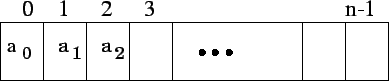
\includegraphics[scale=0.5]{imagens/img18}
\caption{Armazenamento de Lista Sequencial}

\end{figure}

\end{frame}

\begin{frame}
\frametitle{Vantagens em se usar array}

\begin{enumerate}
\item Rápido acesso aos elementos
\item Facilidade em modificar informações
\end{enumerate}
Os elementos do array podem ser acessados em tempo constante, por exemplo, na maioria das linguagens, o elemento que está na posição \textit{i} de um array \textit{a} pode ser recuperado utilizando-se \textit{a[i]}
\end{frame}

\begin{frame}
\frametitle{Desvantagens}
\begin{enumerate}
\item Definição prévia do tamanho do array
\item Dificuldade para inserir (e remover) um elemento entre dois outros já existentes
\end{enumerate}

Na definição de um array precisamos especificar o número máximo de elementos que serão armazenados e manter um registro do número de elementos armazenados 
\end{frame}

\begin{frame}
\frametitle{Inserção}
Suponha que queiramos inserir um novo elemento \textit{x} em uma posição \textit{i} já ocupada de um vetor \textit{a}. Para realizar esta tarefa teremos que deslocar os elementos para as posições seguintes. Note que no pior caso (inserir na primeira posição) esta operação leva tempo \textit{O(n)}. 
\begin{figure}
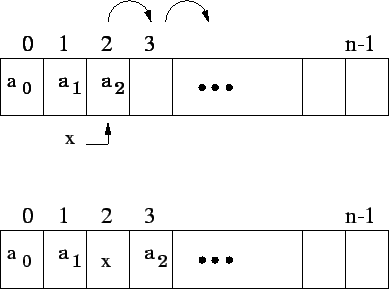
\includegraphics[scale=0.4]{imagens/img21}
\caption{Inserção de elemento}
\end{figure}
\end{frame}

\subsection{2.1 ArrayStack: Operações rápidas usando um Array }
\begin{frame}
\frametitle{Inicialização}
 Um elemento da lista com índice $\ensuremath{\ensuremath{\ensuremath{\mathit{i}}}}$ é armazenado em $\ensuremath{\ensuremath{\ensuremath{\mathit{a}}[\ensuremath{\mathit{i}}]}}$.  Na maioria das vezes, $\ensuremath{\ensuremath{\ensuremath{\mathit{a}}}}$ é maior que o estritamente necessário,
assim um inteiro $\ensuremath{\ensuremath{\ensuremath{\mathit{n}}}}$ é usado para manter um registro do número de elementos realmente armazenados em $\ensuremath{\ensuremath{\ensuremath{\mathit{a}}}}$.  Deste modo, os elementos da lista são armazenados em $
\ensuremath{\ensuremath{\ensuremath{\mathit{a}}[0]}},\ldots,\ensuremath{\ensuremath{\ensuremath{\mathit{a}}[\ensuremath{\mathit{n}}-1]}}$ e, a todo instante, $\ensuremath{\ensuremath{\mathrm{length}(\ensuremath{\mathit{a}})}} \ge \ensuremath{\ensuremath{\ensuremath{\mathit{n}}}}$.

%importing \codeimport{ods/ArrayStack.a.n.size()}: 
\begin{oframed}
\begin{flushleft}
\hspace*{1em} $\ensuremath{\mathrm{initialize}()}$\\
\hspace*{1em} \hspace*{1em} $\ensuremath{\ensuremath{\mathit{a}} \gets  \ensuremath{\mathrm{new\_array}(1)}}$\\
\hspace*{1em} \hspace*{1em} $\ensuremath{\ensuremath{\mathit{n}} \gets  \ensuremath{0}}$\\
\end{flushleft}
\end{oframed}

\end{frame}

\begin{frame}
\frametitle{Operações Básicas}
\begin{oframed}
\begin{flushleft}
\hspace*{1em} $\ensuremath{\mathrm{get}(\ensuremath{\mathit{i}})}$\\

\hspace*{1em} \hspace*{1em} {\color{black} \textbf{return}} $\ensuremath{\ensuremath{\mathit{a}}[\ensuremath{\mathit{i}}]}$\\
\ \\
\hspace*{1em} $\ensuremath{\mathrm{set}(\ensuremath{\mathit{i}}, \ensuremath{\mathit{x}})}$\\

\hspace*{1em} \hspace*{1em} $\ensuremath{\ensuremath{\mathit{y}} \gets  \ensuremath{\ensuremath{\mathit{a}}[\ensuremath{\mathit{i}}]}}$\\
\hspace*{1em} \hspace*{1em} $\ensuremath{\ensuremath{\mathit{a}}[\ensuremath{i}] \gets  \ensuremath{x}}$\\
\hspace*{1em} \hspace*{1em} {\color{black} \textbf{return}} $\ensuremath{\ensuremath{\mathit{y}}}$\\
\end{flushleft}
\end{oframed}
\end{frame}

\begin{frame}
\begin{figure}
  \begin{center}
    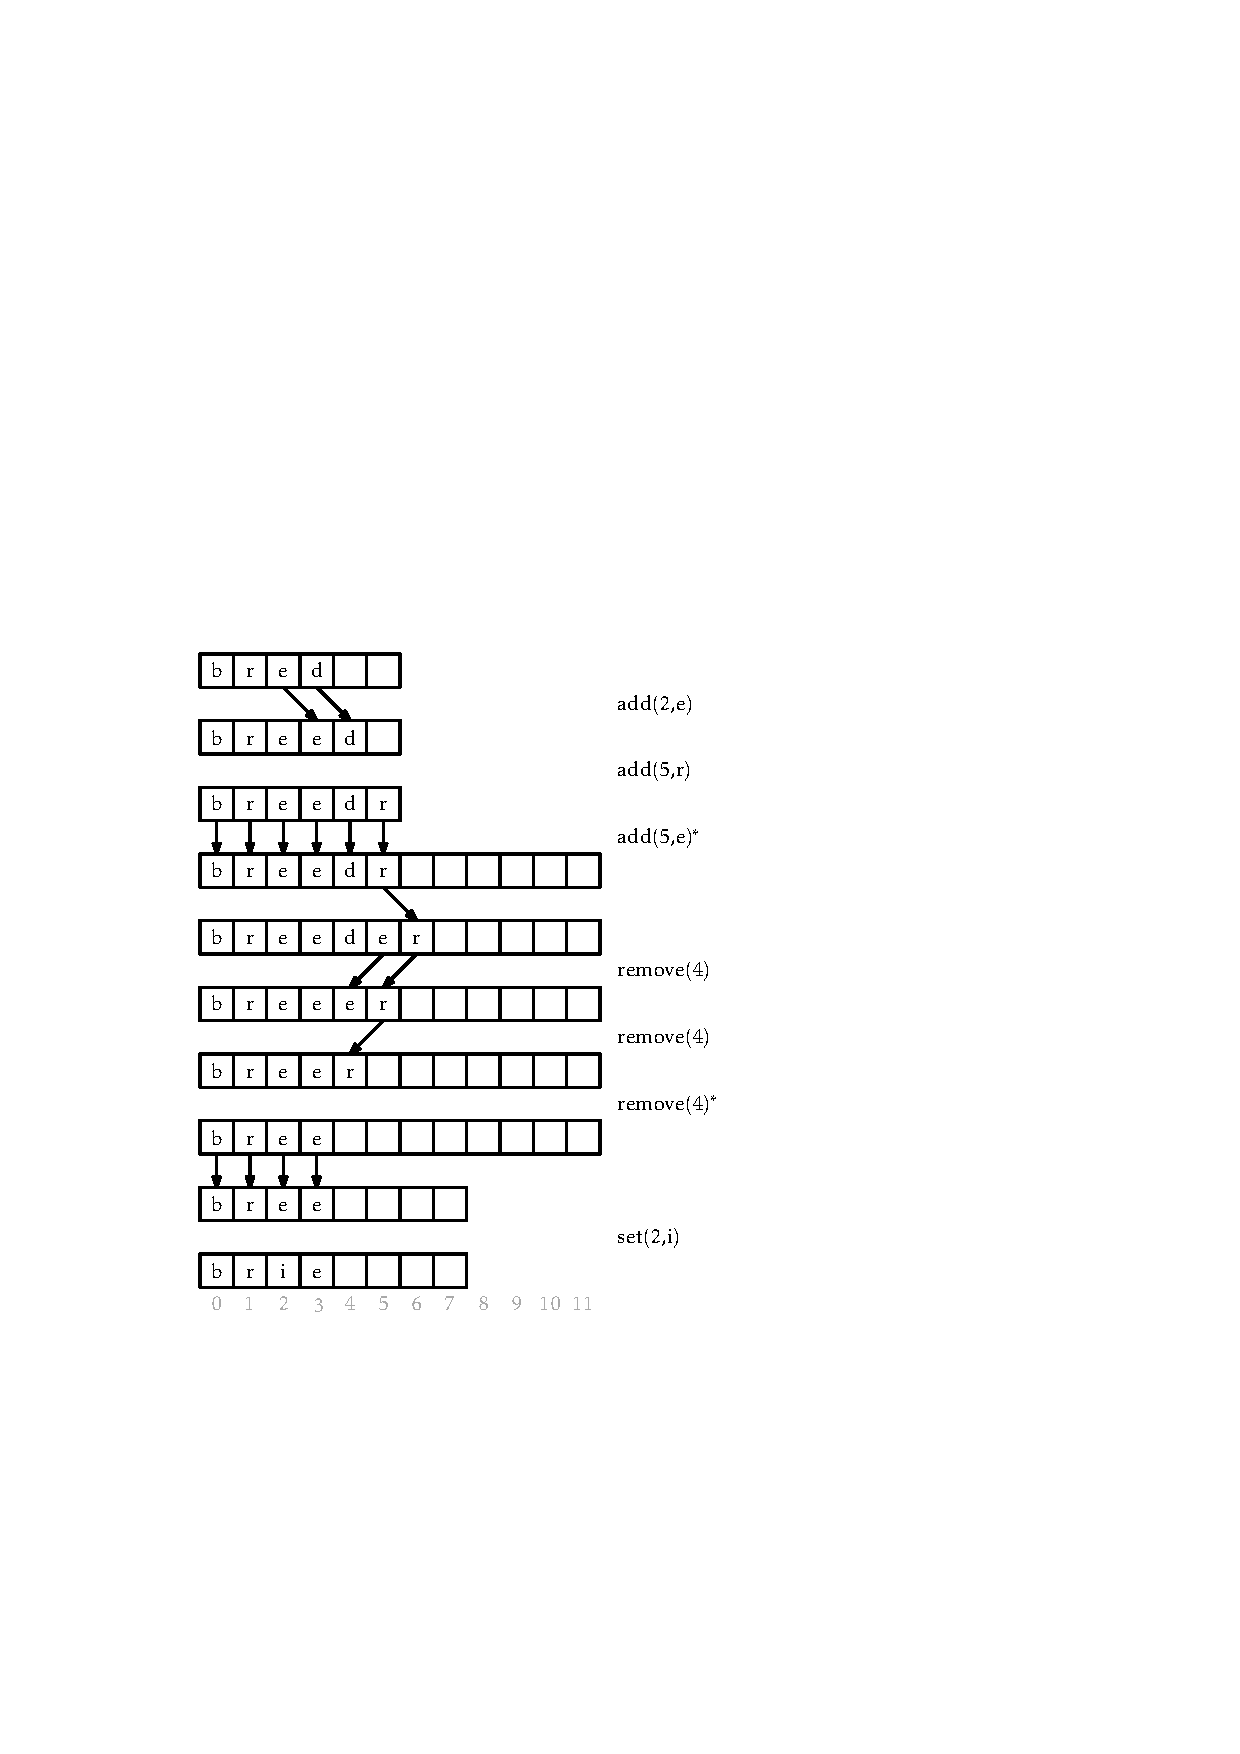
\includegraphics[trim = 0px 172px 0px 0px,clip]{imagens/arraystack}
  \end{center}
  \caption[Adding to an ArrayStack]{Uma sequência de operações $\ensuremath{\ensuremath{\mathrm{add}(\ensuremath{\mathit{i}},\ensuremath{\mathit{x}})}}$  em uma
  ArrayStack.  Setas indicam elementos sendo copiados.  Operações que implicam uma chamada para $\ensuremath{\ensuremath{\mathrm{resize}()}}$ são marcadas com asterisco.}

\end{figure}
\end{frame}

\begin{frame}
\begin{figure}
  \begin{center}
    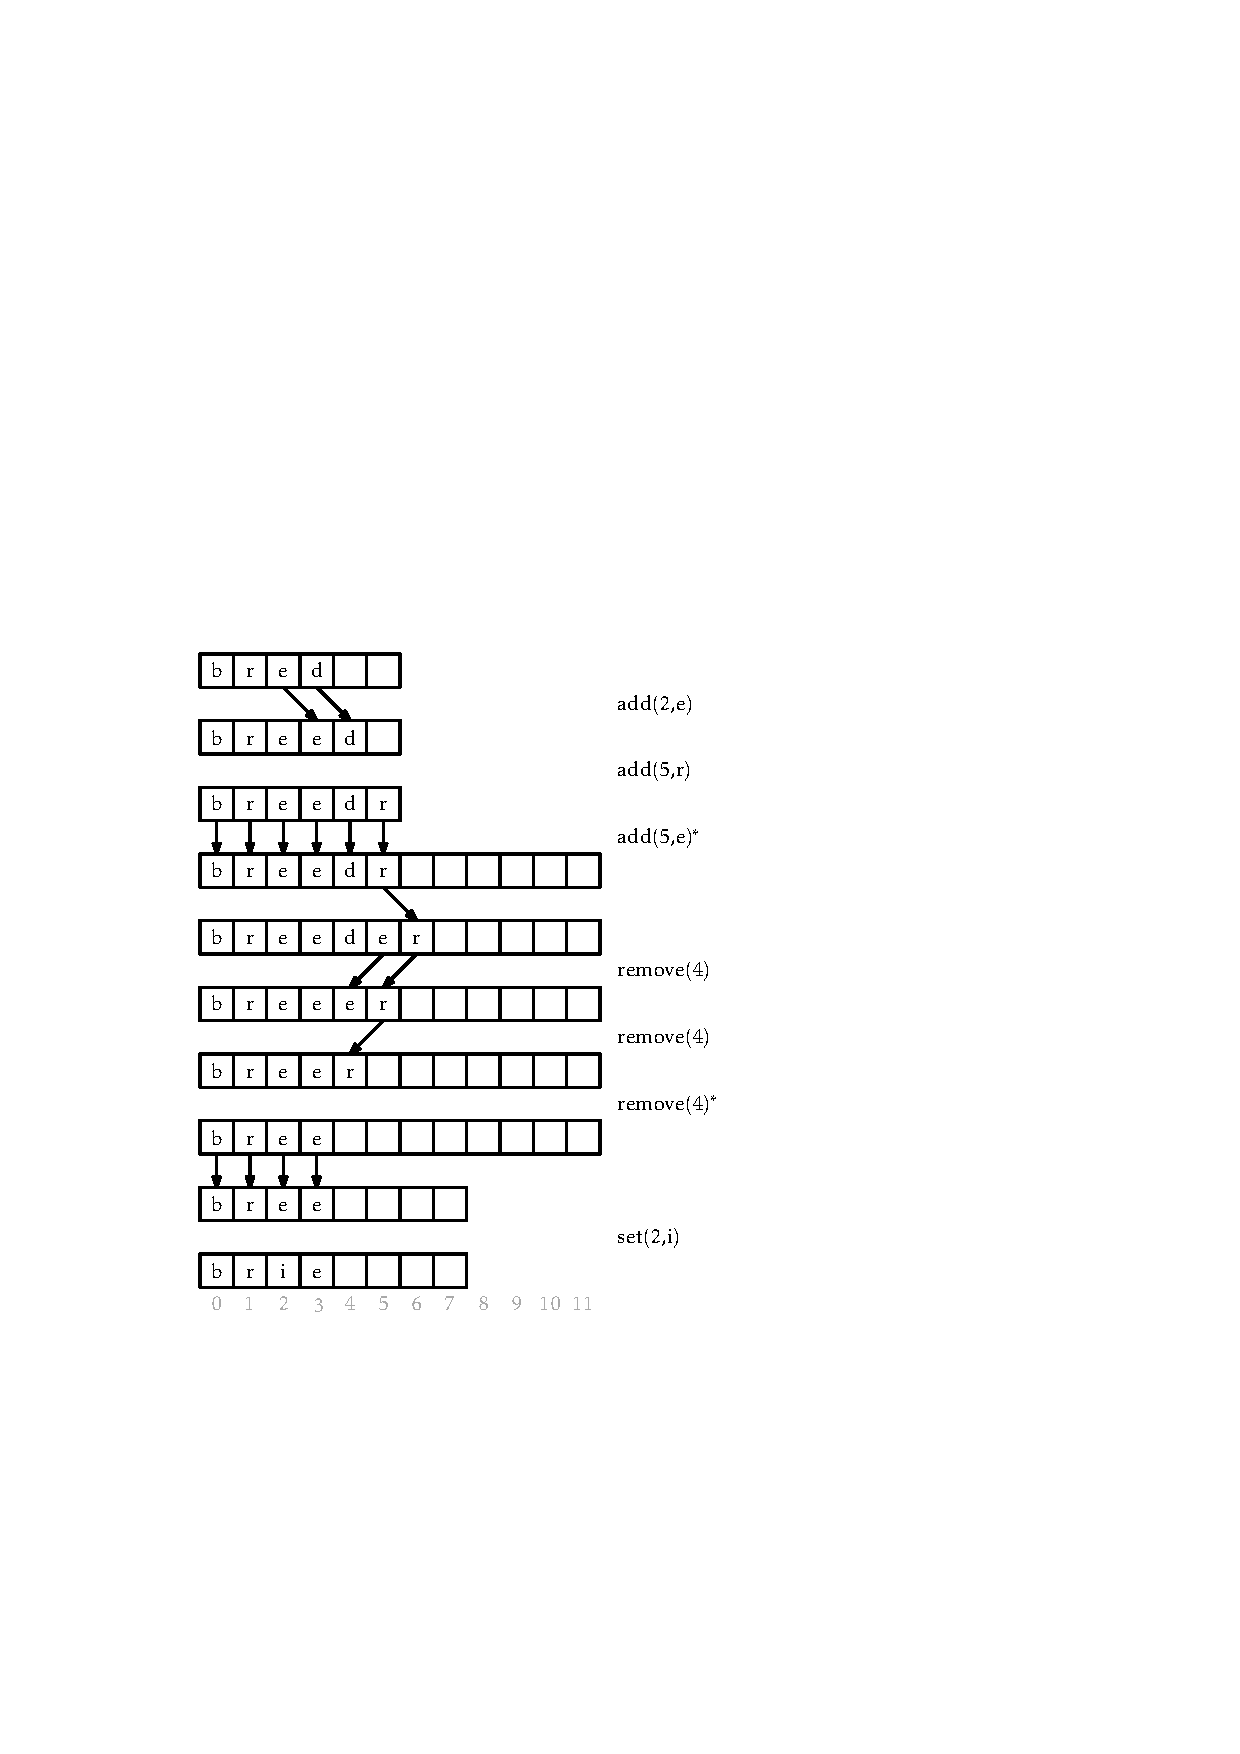
\includegraphics[trim = 0px 0px 0px 130.5px,clip]{imagens/arraystack}
  \end{center}
  \caption[Adding to an ArrayStack]{Uma sequência de operações $\ensuremath{\ensuremath{\mathrm{remove}(\ensuremath{\mathit{i}})}}$.}

\end{figure}
\end{frame}

\begin{frame}
\frametitle{Add}
\begin{oframed}
\begin{flushleft}
\hspace*{1em} $\ensuremath{\mathrm{add}(\ensuremath{\mathit{i}}, \ensuremath{\mathit{x}})}$ \\

\hspace*{1em} \hspace*{1em} {\color{black} \textbf{if}} $\ensuremath{\ensuremath{\mathit{n}} = \mathrm{length}(\ensuremath{\mathit{a}})} {\color{black} \textbf{ then }}  \ensuremath{\mathrm{resize}()}$\\
\hspace*{1em} \hspace*{1em} $\ensuremath{\ensuremath{\mathit{a}}[\ensuremath{\ensuremath{\mathit{i}}+1,\ensuremath{\mathit{i}}+2,\ldots,\ensuremath{n}]} \gets  \ensuremath{\ensuremath{\mathit{a}}[\ensuremath{\ensuremath{\mathit{i}},\ensuremath{\mathit{i}}+1,\ldots,\ensuremath{\mathit{n}}-1}]}}$\\
\hspace*{1em} \hspace*{1em} $\ensuremath{\ensuremath{\mathit{a}}[\ensuremath{i}] \gets  \ensuremath{x}}$\\
\hspace*{1em} \hspace*{1em} $\ensuremath{\ensuremath{\mathit{n}} \gets  \ensuremath{\ensuremath{\mathit{n}} + 1}}$\\
\end{flushleft}
\end{oframed}

Custo da operação (ignorando $\ensuremath{\ensuremath{\mathrm{resize}()}}$) = $O(\ensuremath{\ensuremath{\ensuremath{\mathit{n}}}}-\ensuremath{\ensuremath{\ensuremath{\mathit{i}}}})$
\end{frame}

\begin{frame}
\frametitle{Remove}
\begin{oframed}
\begin{flushleft}
\hspace*{1em} $\ensuremath{\mathrm{remove}(\ensuremath{\mathit{i}})}$ \\

\hspace*{1em} \hspace*{1em} $\ensuremath{\ensuremath{\mathit{x}} \gets  \ensuremath{\ensuremath{\mathit{a}}[\ensuremath{\mathit{i}}]}}$\\
\hspace*{1em} \hspace*{1em} $\ensuremath{\ensuremath{\mathit{a}}[\ensuremath{\ensuremath{\mathit{i}},\ensuremath{\mathit{i}}+1,\ldots,\ensuremath{\ensuremath{\mathit{n}}-2}]} \gets  \ensuremath{\ensuremath{\mathit{a}}[\ensuremath{\ensuremath{\mathit{i}}+1,\ensuremath{\mathit{i}}+2,\ldots,\ensuremath{\mathit{n}}-1}]}}$\\
\hspace*{1em} \hspace*{1em} $\ensuremath{\ensuremath{\mathit{n}} \gets  \ensuremath{\ensuremath{\mathit{n}} - 1}}$\\
\hspace*{1em} \hspace*{1em} {\color{black} \textbf{if}} $\ensuremath{\mathrm{length}(\ensuremath{\mathit{a}}) \ge 3\cdot n}$ {\color{black} \textbf{then}}  $\ensuremath{\mathrm{resize}()}$\\
\hspace*{1em} \hspace*{1em} {\color{black} \textbf{return}} $\ensuremath{\ensuremath{\mathit{x}}}$\\
\end{flushleft}
\end{oframed}
\end{frame}

\begin{frame}
\frametitle{Crescendo e Encolhendo}
\begin{oframed}
\begin{flushleft}
\hspace*{1em} $\ensuremath{\mathrm{resize}()}$\\
\hspace*{1em} \hspace*{1em} $\ensuremath{\ensuremath{\mathit{b}} \gets  \ensuremath{\mathrm{new\_array}(\mathrm{max}(1, 2\cdot \ensuremath{\mathit{n}})})}$\\
\hspace*{1em} \hspace*{1em} $\ensuremath{\ensuremath{\mathit{b}}[\ensuremath{0,1,\ldots,\ensuremath{\ensuremath{\mathit{n}}-1}]} \gets  \ensuremath{\ensuremath{\mathit{a}}[\ensuremath{0,1,\ldots,\ensuremath{\mathit{n}}-1}]}}$\\
\hspace*{1em} \hspace*{1em} $\ensuremath{\ensuremath{\mathit{a}} \gets  \ensuremath{b}}$\\
\end{flushleft}
\end{oframed}
\end{frame}

\begin{frame}

Uma ArrayStack é uma maneira eficiente de implementar uma Stack.
Particularmente, podemos implementar $\ensuremath{\ensuremath{\mathrm{push}(\ensuremath{\mathit{x}})}}$ como $\ensuremath{\ensuremath{\mathrm{add}(\ensuremath{\mathit{n}},\ensuremath{\mathit{x}})}}$ e $\ensuremath{\ensuremath{\mathrm{pop}()}}$
como  $\ensuremath{\ensuremath{\mathrm{remove}(\ensuremath{\mathit{n}}-1)}}$, em cada caso, estas operações executaram em um tempo amortizado de $O(1)$.

\end{frame}

\subsection{2.2 Cópia otimizada de Array}
\begin{frame}
\frametitle{2.2 Cópia otimizada de Array}

Algumas linguagens permitem uma cópia otimizada de áreas de memória, acelerando a operação de resize. Na linguagem C
temos as funções $\ensuremath{\ensuremath{\mathrm{memcpy}(\ensuremath{\mathit{d}},\ensuremath{\mathit{s}},\ensuremath{\mathit{n}})}}$ e $\ensuremath{\ensuremath{\mathrm{memmove}(\ensuremath{\mathit{d}},\ensuremath{\mathit{s}},\ensuremath{\mathit{n}})}}$. Na linguagem C++ temos $\ensuremath{\ensuremath{\mathrm{stdcopy}(\ensuremath{\mathit{a_0}},\ensuremath{\mathit{a_1}},\ensuremath{\mathit{b}})}}$.
Java possui o método $\ensuremath{\ensuremath{\mathrm{System}.\mathrm{arraycopy}(\ensuremath{\mathit{s}},\ensuremath{\mathit{i}},\ensuremath{\mathit{d}},\ensuremath{\mathit{j}},\ensuremath{\mathit{n}})}}$.

\end{frame}

\subsection{2.3 Fila Baseada em Array}
\begin{frame}
\frametitle{2.3 Fila Baseada em Array}
A estrutura ArrayQueue implementa uma fila FIFO (first-in-first-out) na qual os elementos são removidos (usando
a operação $\ensuremath{\ensuremath{\mathrm{remove}()}}$) da fila na mesma ordem em que são inseridos (usando a operação $\ensuremath{\ensuremath{\mathrm{add}(\ensuremath{\mathit{x}})}}$).


\end{frame}

\begin{frame}
\frametitle{Como implementar?}

Por que não ArrayStack?

\end{frame}

\begin{frame}
\frametitle{Como implementar?}

Array infinito? Com $j$ indicando o elemento a ser removido e $n$ o número de elementos na Fila.


Os elementos são armazenados em:

$[a[j],a[j+1],\ldots,a[j+n-1] \enspace]$

Inicialmente, ambos $j$ e $n$ são 0.  Para acrescentar um elemento, devemos colocá-lo em $a[j+n]$ e incrementar $\ensuremath{\ensuremath{\ensuremath{\mathit{n}}}}$.
Para remover um elemento, devemos removê-lo de $\ensuremath{\ensuremath{\ensuremath{\mathit{a}}[\ensuremath{\mathit{j}}]}}$, incrementar $\ensuremath{\ensuremath{\ensuremath{\mathit{j}}}}$, e
decrementar $\ensuremath{\ensuremath{\ensuremath{\mathit{n}}}}$.

\end{frame}

\begin{frame}
Qual o problema desta solução?

\end{frame}

\begin{frame}
\frametitle{Aritmética modular}

 Podemos simular um Array infinito usando um array finito $a$
e \emph{aritmética modular}.

Esta também é chamada de aritmética do relógio.  Por exemplo 10:00 mais cinco dá 3:00.  Formalmente, dizemos que
\[
    10 + 5 = 15 \equiv 3 \pmod{12} \enspace .
\]
Que lemos como ``15 é congruente a 3 módulo
12.'' Também podemos tratar $\bmod$ como um operador, de modo que
\[
   15 \bmod 12 = 3 \enspace .
\]

\end{frame}

\begin{frame}
\frametitle{Array finito tratado como infinito}

As posições passam  a ser:
 $a[j \bmod length(a)],a[(j+1) \bmod length(a)],\ldots,a[(j+n-1) \bmod a)]
\enspace.]$

Isto trata o Array $a$ como um Array \emph{circular}
cujos índices que são maiores que $length(a)-1$ ``voltam'' ao início do array.
\end{frame}

\begin{frame}
\frametitle{Inicialização}
\begin{oframed}
\begin{flushleft}
\hspace*{1em} $\ensuremath{\mathrm{initialize}()}$\\
\hspace*{1em} \hspace*{1em} $\ensuremath{\ensuremath{\mathit{a}} \gets  \ensuremath{\mathrm{new\_array}(1)}}$\\
\hspace*{1em} \hspace*{1em} $\ensuremath{\ensuremath{\mathit{j}} \gets  \ensuremath{0}}$\\
\hspace*{1em} \hspace*{1em} $\ensuremath{\ensuremath{\mathit{n}} \gets  \ensuremath{0}}$\\
\end{flushleft}
\end{oframed}
\end{frame}

\begin{frame}
\frametitle{Inserindo e removendo de um ArrayQueue}
\begin{figure}
  \begin{center}
    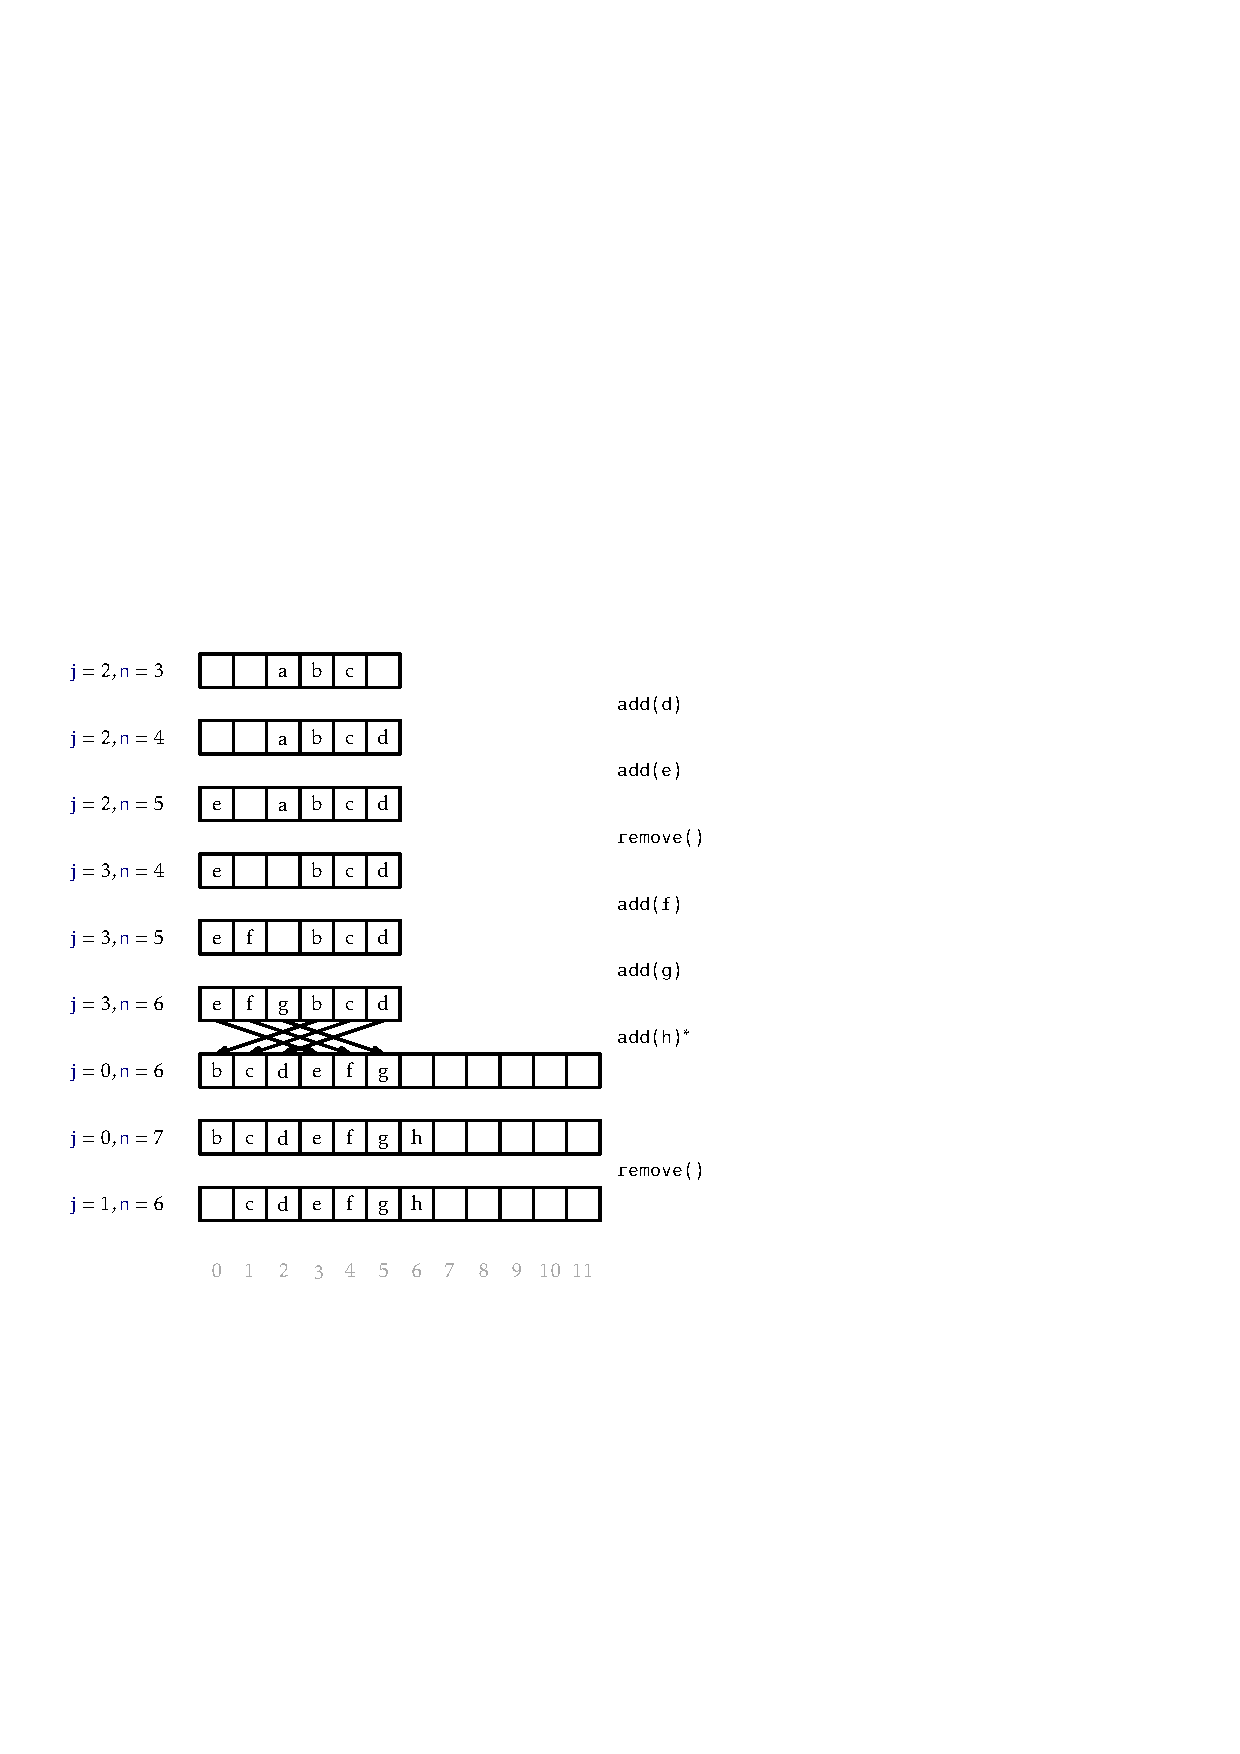
\includegraphics[scale=0.90909, trim=0px 155px 0px 0px, clip]{imagens/arrayqueue}
  \end{center}
  \caption[Inserindo e removendo de um ArrayQueue]{Uma sequência de $\ensuremath{\ensuremath{\mathrm{add}(\ensuremath{\mathit{x}})}}$ e $\ensuremath{\ensuremath{\mathrm{remove}(\ensuremath{\mathit{i}})}}$.}
\end{figure}
\end{frame}

\begin{frame}
\frametitle{Inserindo e removendo de um ArrayQueue}
\begin{figure}
  \begin{center}
    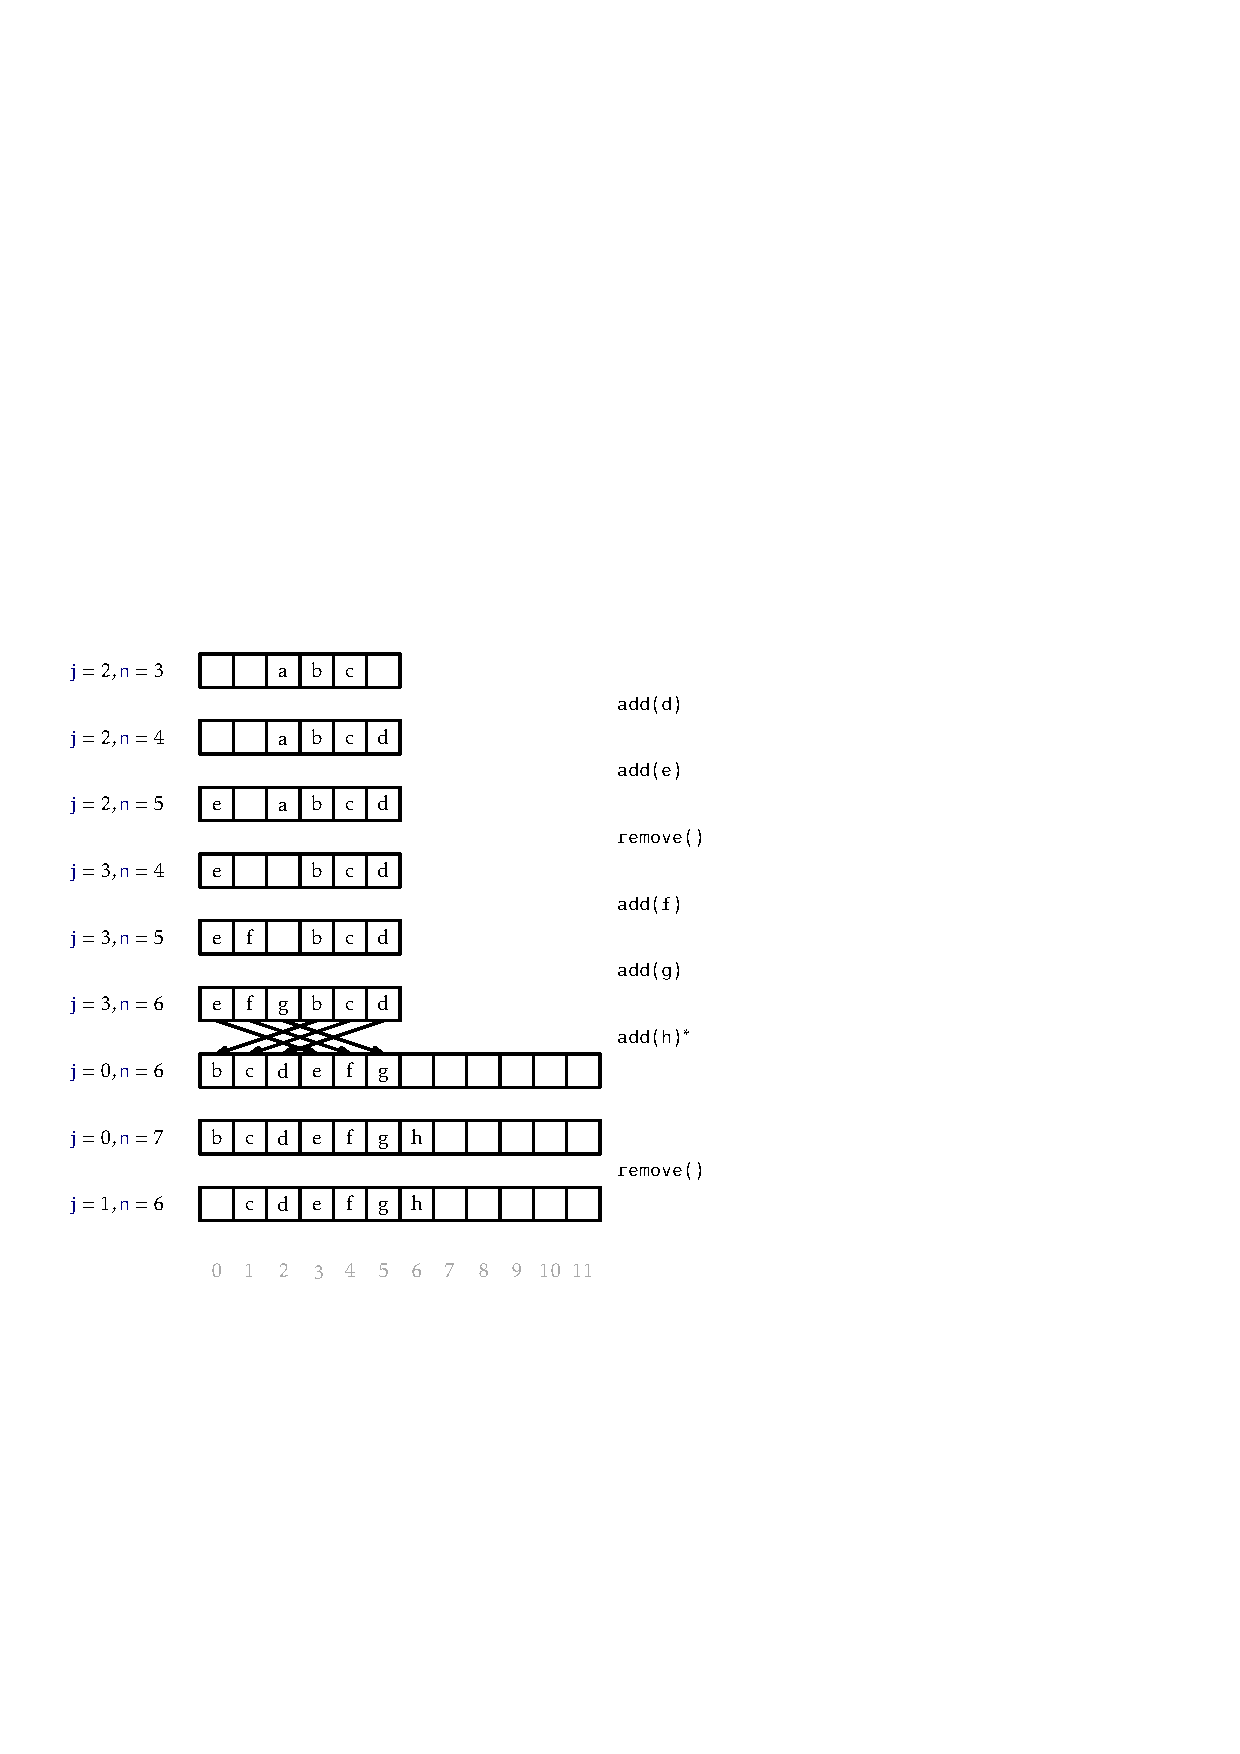
\includegraphics[scale=0.90909, trim=0px 0px 0px 130px, clip]{imagens/arrayqueue}
  \end{center}
 \caption[Inserindo e removendo de um ArrayQueue]{Uma sequência de $\ensuremath{\ensuremath{\mathrm{add}(\ensuremath{\mathit{x}})}}$ e $\ensuremath{\ensuremath{\mathrm{remove}(\ensuremath{\mathit{i}})}}$.}
\end{figure}
\end{frame}

\begin{frame}
\frametitle{$Add()$}
\begin{oframed}
\begin{flushleft}
\hspace*{1em} $\ensuremath{\mathrm{add}(\ensuremath{\mathit{x}})}$\\
\hspace*{1em} \hspace*{1em} {\color{black} \textbf{if}} $\ensuremath{\ensuremath{\mathit{n}} + 1 > \mathrm{length}(\ensuremath{\mathit{a}})} {\color{black} \textbf{ then }}  \ensuremath{\mathrm{resize}()}$\\
\hspace*{1em} \hspace*{1em} $\ensuremath{\ensuremath{\mathit{a}}[\ensuremath{(\ensuremath{\mathit{j}}+\ensuremath{\mathit{n}}) \bmod  \mathrm{length}(\ensuremath{\mathit{a}})}] \gets  \ensuremath{x}}$\\
\hspace*{1em} \hspace*{1em} $\ensuremath{\ensuremath{\mathit{n}} \gets  \ensuremath{\ensuremath{\mathit{n}} + 1}}$\\
\hspace*{1em} \hspace*{1em} {\color{black} \textbf{return}} $\ensuremath{\ensuremath{\mathit{true}}}$\\
\end{flushleft}
\end{oframed}
\end{frame}

\begin{frame}
\frametitle{$remove()$}
\begin{oframed}
\begin{flushleft}
\hspace*{1em} $\ensuremath{\mathrm{remove}()}$\\

\hspace*{1em} \hspace*{1em} $\ensuremath{\ensuremath{\mathit{x}} \gets  \ensuremath{\ensuremath{\mathit{a}}[\ensuremath{\mathit{j}}]}}$\\
\hspace*{1em} \hspace*{1em} $\ensuremath{\ensuremath{\mathit{j}} \gets  \ensuremath{(\ensuremath{\mathit{j}} + 1) \bmod  \mathrm{length}(\ensuremath{\mathit{a}})}}$\\
\hspace*{1em} \hspace*{1em} $\ensuremath{\ensuremath{\mathit{n}} \gets  \ensuremath{\ensuremath{\mathit{n}} - 1}}$\\
\hspace*{1em} \hspace*{1em} {\color{black} \textbf{if}} $\ensuremath{\mathrm{length}(\ensuremath{\mathit{a}}) \ge 3\cdot n} {\color{black} \textbf{ then }}  \ensuremath{\mathrm{resize}()}$\\
\hspace*{1em} \hspace*{1em} {\color{black} \textbf{return}} $\ensuremath{\ensuremath{\mathit{x}}}$\\
\end{flushleft}
\end{oframed}
\end{frame}

\begin{frame}
\frametitle{$resize()$}
\begin{oframed}
\begin{flushleft}
\hspace*{1em} $\ensuremath{\mathrm{resize}()}$\\
\hspace*{1em} \hspace*{1em} $\ensuremath{\ensuremath{\mathit{b}} \gets  \ensuremath{\mathrm{new\_array}(\mathrm{max}(1, 2\cdot \ensuremath{\mathit{n}})})}$\\
\hspace*{1em} \hspace*{1em} {\color{black} \textbf{for}} $\ensuremath{k}$ {\color{black} \textbf{in}} $\ensuremath{0,1,2,\ldots,\ensuremath{\mathit{n}}-1} {\color{black} \textbf{do}}$ \\
\hspace*{1em} \hspace*{1em} \hspace*{1em} $\ensuremath{\ensuremath{\mathit{b}}[\ensuremath{k}] \gets  \ensuremath{\ensuremath{\mathit{a}}[(\ensuremath{\mathit{j}}+\ensuremath{\mathit{k}}) \bmod  \mathrm{length}(\ensuremath{\mathit{a}})]}}$\\
\hspace*{1em} \hspace*{1em} $\ensuremath{\ensuremath{\mathit{a}} \gets  \ensuremath{b}}$\\
\hspace*{1em} \hspace*{1em} $\ensuremath{\ensuremath{\mathit{j}} \gets  \ensuremath{0}}$\\
\end{flushleft}
\end{oframed}
\end{frame}

\subsection{2.4 ArrayDeque}
\begin{frame}
\frametitle{$Inicialize()$}
Usando a mesma estrutura circular.
\begin{oframed}
\begin{flushleft}
\hspace*{1em} $\ensuremath{\mathrm{initialize}()}$\\
\hspace*{1em} \hspace*{1em} $\ensuremath{\ensuremath{\mathit{a}} \gets  \ensuremath{\mathrm{new\_array}(1)}}$\\
\hspace*{1em} \hspace*{1em} $\ensuremath{\ensuremath{\mathit{j}} \gets  \ensuremath{0}}$\\
\hspace*{1em} \hspace*{1em} $\ensuremath{\ensuremath{\mathit{n}} \gets  \ensuremath{0}}$\\
\end{flushleft}
\end{oframed}
\end{frame}

\begin{frame}
\frametitle{$Get()$ e $Set()$}
\begin{oframed}
\begin{flushleft}
\hspace*{1em} $\ensuremath{\mathrm{get}(\ensuremath{\mathit{i}})}$\\

\hspace*{1em} \hspace*{1em} {\color{black} \textbf{return}} $\ensuremath{\ensuremath{\mathit{a}}[(\ensuremath{\mathit{i}}+\ensuremath{\mathit{j}})\bmod \mathrm{length}(\ensuremath{\mathit{a}})]}$\\
\ \\
\hspace*{1em} $\ensuremath{\mathrm{set}(\ensuremath{\mathit{i}}, \ensuremath{\mathit{x}})}$\\

\hspace*{1em} \hspace*{1em} $\ensuremath{\ensuremath{\mathit{y}} \gets  \ensuremath{\ensuremath{\mathit{a}}[(\ensuremath{\mathit{i}}+\ensuremath{\mathit{j}})\bmod \mathrm{length}(\ensuremath{\mathit{a}})]}}$\\
\hspace*{1em} \hspace*{1em} $\ensuremath{\ensuremath{\mathit{a}}[\ensuremath{(\ensuremath{\mathit{i}}+\ensuremath{\mathit{j}})\bmod \mathrm{length}(\ensuremath{\mathit{a}})}] \gets  \ensuremath{x}}$\\
\hspace*{1em} \hspace*{1em} {\color{black} \textbf{return}} $\ensuremath{\ensuremath{\mathit{y}}}$\\
\end{flushleft}
\end{oframed}
\end{frame}

\begin{frame}
\frametitle{}
\begin{figure}
  \begin{center}
    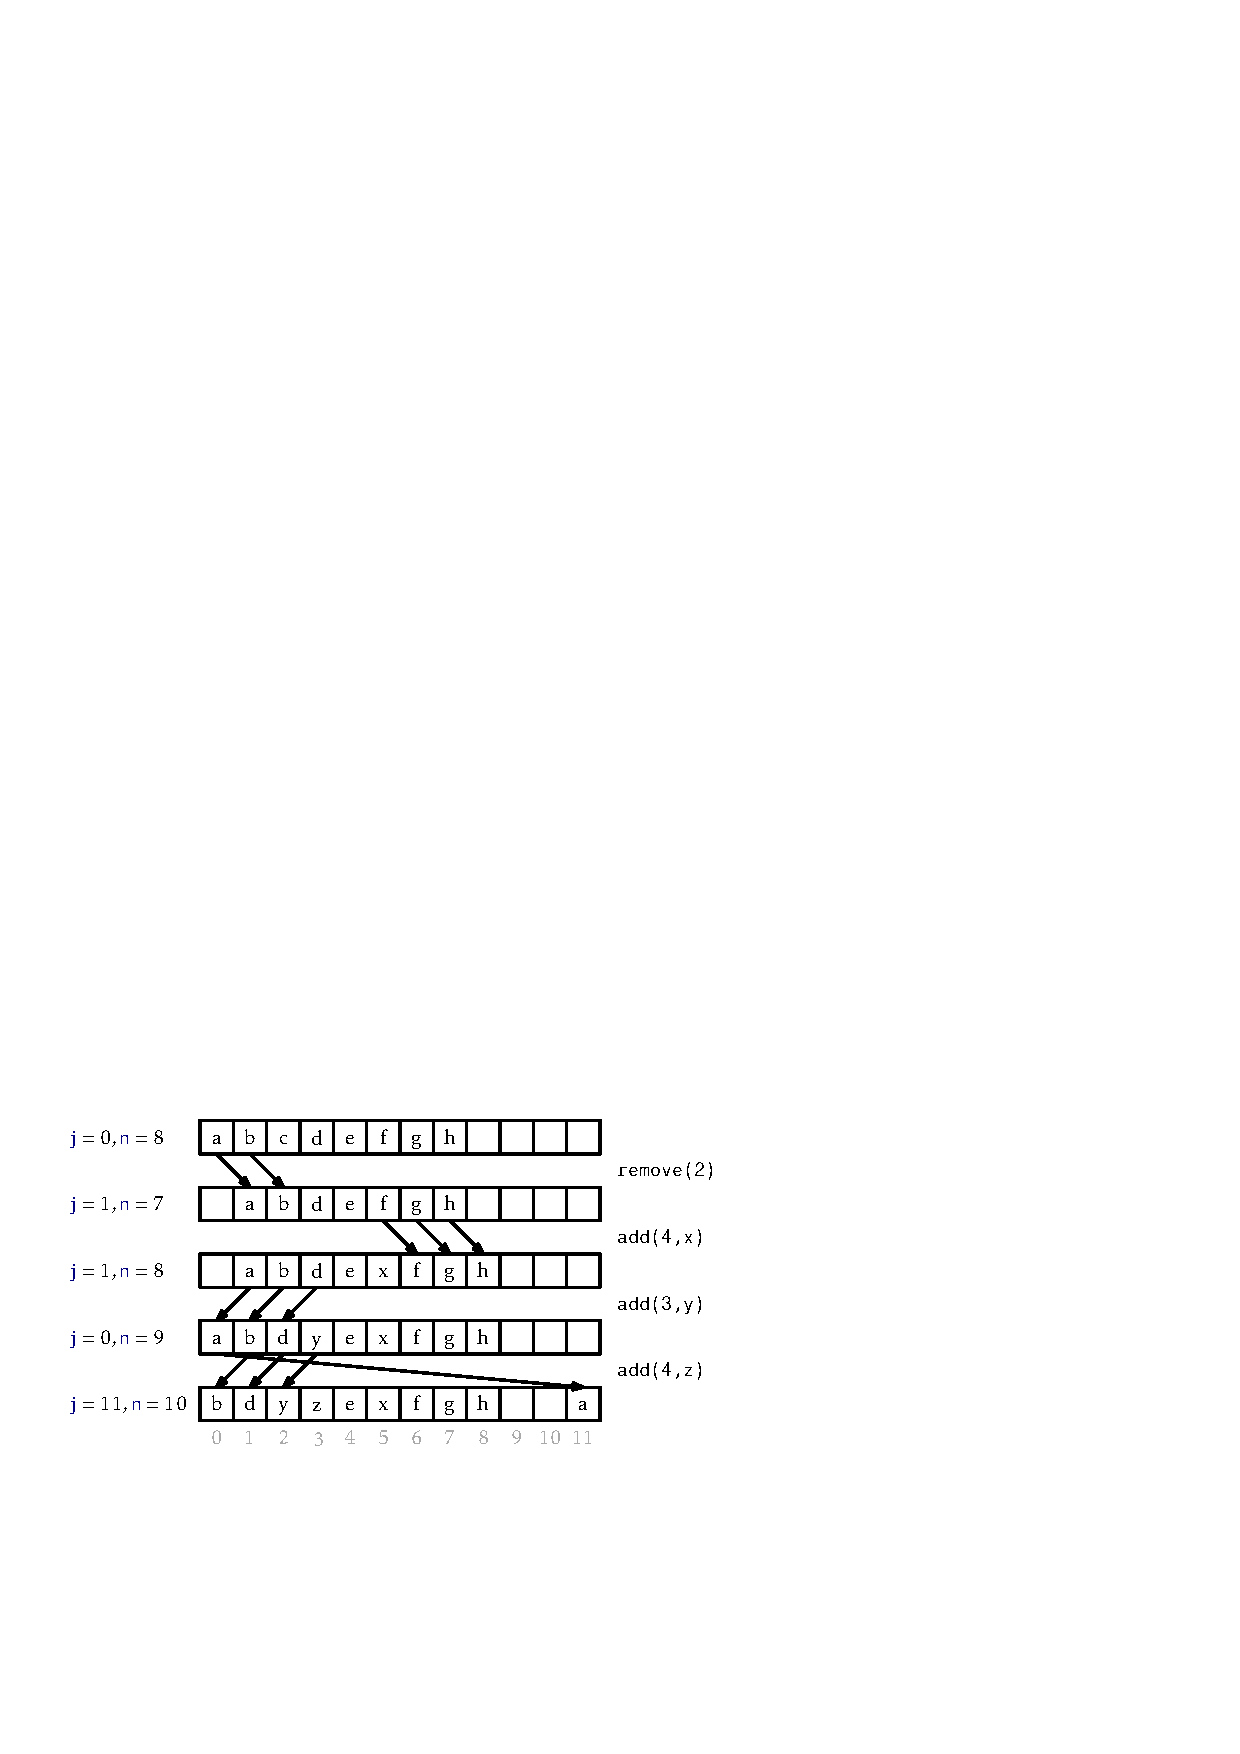
\includegraphics[scale=0.90909]{imagens/arraydeque}
  \end{center}
  \caption[Adding and removing from an ArrayDeque]{Uma sequência de operações $\ensuremath{\ensuremath{\mathrm{add}(\ensuremath{\mathit{i}},\ensuremath{\mathit{x}})}}$ e $\ensuremath{\ensuremath{\mathrm{remove}(\ensuremath{\mathit{i}})}}$ sobre um
  ArrayDeque.}
\end{figure}
\end{frame}

\begin{frame}
\frametitle{$Add(i,x)$}
\begin{oframed}
\begin{flushleft}
\hspace*{1em} $\ensuremath{\mathrm{add}(\ensuremath{\mathit{i}}, \ensuremath{\mathit{x}})}$ \\

\hspace*{1em} \hspace*{1em} {\color{black} \textbf{if}} $\ensuremath{\ensuremath{\mathit{n}} = \mathrm{length}(\ensuremath{\mathit{a}})}$ {\color{black} \textbf{then}}  $\ensuremath{\mathrm{resize}()}$\\
\hspace*{1em} \hspace*{1em} {\color{black} \textbf{if}} $\ensuremath{\ensuremath{\mathit{i}} < \ensuremath{\mathit{n}}/2}$ {\color{black} \textbf{then}} \\
\hspace*{1em} \hspace*{1em} \hspace*{1em} $\ensuremath{\ensuremath{\mathit{j}} \gets  \ensuremath{(\ensuremath{\mathit{j}}-1) \bmod  \mathrm{length}(\ensuremath{\mathit{a}})}}$\\
\hspace*{1em} \hspace*{1em} \hspace*{1em} {\color{black} \textbf{for}} $\ensuremath{k}$ {\color{black} \textbf{in}} $\ensuremath{0,1,2,\ldots,\ensuremath{\mathit{i}}-1}$ {\color{black} \textbf{do}} \\
\hspace*{1em} \hspace*{1em} \hspace*{1em} \hspace*{1em} $\ensuremath{\ensuremath{\mathit{a}}[\ensuremath{(\ensuremath{\mathit{j}}+\ensuremath{\mathit{k}})\bmod \mathrm{length}(\ensuremath{\mathit{a}})}] \gets  \ensuremath{\ensuremath{\mathit{a}}[(\ensuremath{\mathit{j}}+\ensuremath{\mathit{k}}+1)\bmod \mathrm{length}(\ensuremath{\mathit{a}})]}}$\\
\hspace*{1em} \hspace*{1em} {\color{black} \textbf{else}} \\
\hspace*{1em} \hspace*{1em} \hspace*{1em} {\color{black} \textbf{for}} $\ensuremath{k}$ {\color{black} \textbf{in}} $\ensuremath{\ensuremath{\mathit{n}},\ensuremath{\mathit{n}}-1,\ensuremath{\mathit{n}}-2,\ldots,\ensuremath{\mathit{i}}+1}$ {\color{black} \textbf{do}} \\
\hspace*{1em} \hspace*{1em} \hspace*{1em} \hspace*{1em} $\ensuremath{\ensuremath{\mathit{a}}[\ensuremath{(\ensuremath{\mathit{j}}+\ensuremath{\mathit{k}})\bmod \mathrm{length}(\ensuremath{\mathit{a}})}] \gets  \ensuremath{\ensuremath{\mathit{a}}[(\ensuremath{\mathit{j}}+\ensuremath{\mathit{k}}-1)\bmod \mathrm{length}(\ensuremath{\mathit{a}})]}}$\\
\hspace*{1em} \hspace*{1em} $\ensuremath{\ensuremath{\mathit{a}}[\ensuremath{(\ensuremath{\mathit{j}}+\ensuremath{\mathit{i}})\bmod \mathrm{length}(\ensuremath{\mathit{a}})}] \gets  \ensuremath{x}}$\\
\hspace*{1em} \hspace*{1em} $\ensuremath{\ensuremath{\mathit{n}} \gets  \ensuremath{\ensuremath{\mathit{n}} + 1}}$\\
\end{flushleft}
\end{oframed}
\end{frame}

\begin{frame}
\frametitle{$remove()$}
\begin{oframed}
\begin{flushleft}
\hspace*{1em} $\ensuremath{\mathrm{remove}(\ensuremath{\mathit{i}})}$ \\

\hspace*{1em} \hspace*{1em} $\ensuremath{\ensuremath{\mathit{x}} \gets  \ensuremath{\ensuremath{\mathit{a}}[(\ensuremath{\mathit{j}}+\ensuremath{\mathit{i}})\bmod \mathrm{length}(\ensuremath{\mathit{a}})]}}$\\
\hspace*{1em} \hspace*{1em} {\color{black} \textbf{if}} $\ensuremath{\ensuremath{\mathit{i}} < \ensuremath{\mathit{n}} / 2}$ {\color{black} \textbf{then}} \\
\hspace*{1em} \hspace*{1em} \hspace*{1em} {\color{black} \textbf{for}} $\ensuremath{k}$ {\color{black} \textbf{in}} $\ensuremath{\ensuremath{\mathit{i}},\ensuremath{\mathit{i}}-1,\ensuremath{\mathit{i}}-2,\ldots,1}$ {\color{black} \textbf{do}} \\
\hspace*{1em} \hspace*{1em} \hspace*{1em} \hspace*{1em} $\ensuremath{\ensuremath{\mathit{a}}[\ensuremath{(\ensuremath{\mathit{j}}+\ensuremath{\mathit{k}})\bmod \mathrm{length}(\ensuremath{\mathit{a}})}] \gets  \ensuremath{\ensuremath{\mathit{a}}[(\ensuremath{\mathit{j}}+\ensuremath{\mathit{k}}-1)\bmod \mathrm{length}(\ensuremath{\mathit{a}})]}}$\\
\hspace*{1em} \hspace*{1em} \hspace*{1em} $\ensuremath{\ensuremath{\mathit{j}} \gets  \ensuremath{(\ensuremath{\mathit{j}}+1) \bmod  \mathrm{length}(\ensuremath{\mathit{a}})}}$\\
\hspace*{1em} \hspace*{1em} {\color{black} \textbf{else}} \\
\hspace*{1em} \hspace*{1em} \hspace*{1em} {\color{black} \textbf{for}} $\ensuremath{k}$ {\color{black} \textbf{in}} $\ensuremath{\ensuremath{\mathit{i}},\ensuremath{\mathit{i}}+1,\ensuremath{\mathit{i}}+2,\ldots,\ensuremath{\mathit{n}}-2}$ {\color{black} \textbf{do}}  \\
\hspace*{1em} \hspace*{1em} \hspace*{1em} \hspace*{1em} $\ensuremath{\ensuremath{\mathit{a}}[\ensuremath{(\ensuremath{\mathit{j}}+\ensuremath{\mathit{k}})\bmod \mathrm{length}(\ensuremath{\mathit{a}})}] \gets  \ensuremath{\ensuremath{\mathit{a}}[(\ensuremath{\mathit{j}}+\ensuremath{\mathit{k}}+1)\bmod \mathrm{length}(\ensuremath{\mathit{a}})]}}$\\
\hspace*{1em} \hspace*{1em} $\ensuremath{\ensuremath{\mathit{n}} \gets  \ensuremath{\ensuremath{\mathit{n}} - 1}}$\\
\hspace*{1em} \hspace*{1em} {\color{black} \textbf{if}} $\ensuremath{\mathrm{length}(\ensuremath{\mathit{a}}) \ge 3\cdot n}$ {\color{black} \textbf{then}}  $\ensuremath{\mathrm{resize}()}$\\
\hspace*{1em} \hspace*{1em} {\color{black} \textbf{return}} $\ensuremath{\ensuremath{\mathit{x}}}$\\
\end{flushleft}
\end{oframed}
\end{frame}

\begin{frame}
\frametitle{Implementando ArrayDeque}
  \begin{itemize}
    \item $\ensuremath{\ensuremath{\mathrm{get}(\ensuremath{\mathit{i}})}}$ e $\ensuremath{\ensuremath{\mathrm{set}(\ensuremath{\mathit{i}},\ensuremath{\mathit{x}})}}$ em $O(1)$ tempo por operação e
    \item $\ensuremath{\ensuremath{\mathrm{add}(\ensuremath{\mathit{i}},\ensuremath{\mathit{x}})}}$ and $\ensuremath{\ensuremath{\mathrm{remove}(\ensuremath{\mathit{i}})}}$ em um tempo $O(1+\min\{\ensuremath{\ensuremath{\ensuremath{\mathit{i}}}},\ensuremath{\ensuremath{\ensuremath{\mathit{n}}}}-\ensuremath{\ensuremath{\ensuremath{\mathit{i}}}}\})$  por operação.
  \end{itemize}
\end{frame}

\subsection{2.5 DualArrayDeque}
\begin{frame}
\frametitle{Construindo uma fila com duas pilhas}

Uma DualArrayDeque usa duas ArrayStack para contruir uma lista.
\end{frame}

\begin{frame}
\frametitle{$Inicialize()$}
\begin{oframed}
\begin{flushleft}
\hspace*{1em} $\ensuremath{\mathrm{initialize}()}$\\
\hspace*{1em} \hspace*{1em} $\ensuremath{\ensuremath{\mathit{front}} \gets  \ensuremath{\mathrm{\mathrm{ArrayStack}}()}}$\\
\hspace*{1em} \hspace*{1em} $\ensuremath{\ensuremath{\mathit{back}} \gets  \ensuremath{\mathrm{\mathrm{ArrayStack}}()}}$\\
\end{flushleft}
\end{oframed}
\end{frame}

\begin{frame}
\frametitle{$size()$}
\begin{oframed}
\begin{flushleft}
\hspace*{1em} $\ensuremath{\mathrm{size}()}$\\
\hspace*{1em} \hspace*{1em} {\color{black} \textbf{return}} $\ensuremath{\ensuremath{\mathit{front}}.\mathrm{size}() + \ensuremath{\mathit{back}}.\mathrm{size}()}$\\
\end{flushleft}
\end{oframed}
\end{frame}

\begin{frame}
\frametitle{}
A pilha $front$ armazena os elementos cujos índice são $0,\ldots,\ensuremath{\ensuremath{\ensuremath{\mathit{front}}.\mathrm{size}()}}-1$, mas o faz na ordem reversa.
A pilha $back$ contém a lista com os elementos de índices $\ensuremath{\ensuremath{\ensuremath{\mathit{front}}.\mathrm{size}()}},\ldots,\ensuremath{\ensuremath{\mathrm{size}()}}-1$ na ordem normal.  Deste modo,
$\ensuremath{\ensuremath{\mathrm{get}(\ensuremath{\mathit{i}})}}$ e $\ensuremath{\ensuremath{\mathrm{set}(\ensuremath{\mathit{i}},\ensuremath{\mathit{x}})}}$ traduzem nas chamadas apropriadas para $\ensuremath{\ensuremath{\mathrm{get}(\ensuremath{\mathit{i}})}}$
ou $\ensuremath{\ensuremath{\mathrm{set}(\ensuremath{\mathit{i}},\ensuremath{\mathit{x}})}}$ nas respectivas $\ensuremath{\ensuremath{\ensuremath{\mathit{front}}}}$ ou $\ensuremath{\ensuremath{\ensuremath{\mathit{back}}}}$, com um tempo de $O(1)$ por operação.
\end{frame}

\begin{frame}
\frametitle{$get()$ e $set()$}
\begin{oframed}
\begin{flushleft}
\hspace*{1em} $\ensuremath{\mathrm{get}(\ensuremath{\mathit{i}})}$\\
\hspace*{1em} \hspace*{1em} {\color{black} \textbf{if}} $\ensuremath{\ensuremath{\mathit{i}} < \ensuremath{\mathit{front}}.\mathrm{size}()}$ {\color{black} \textbf{then}} \\
\hspace*{1em} \hspace*{1em} \hspace*{1em} {\color{black} \textbf{return}} $\ensuremath{\ensuremath{\mathit{front}}.\mathrm{get}(\ensuremath{\mathit{front}}.\mathrm{size}()-\ensuremath{\mathit{i}}-1})$\\
\hspace*{1em} \hspace*{1em} {\color{black} \textbf{else}} \\
\hspace*{1em} \hspace*{1em} \hspace*{1em} {\color{black} \textbf{return}} $\ensuremath{\ensuremath{\mathit{back}}.\mathrm{get}(\ensuremath{\mathit{i}}-\ensuremath{\mathit{front}}.\mathrm{size}()})$\\
\ \\
\hspace*{1em} $\ensuremath{\mathrm{set}(\ensuremath{\mathit{i}}, \ensuremath{\mathit{x}})}$\\
\hspace*{1em} \hspace*{1em} {\color{black} \textbf{if}} $\ensuremath{\ensuremath{\mathit{i}} < \ensuremath{\mathit{front}}.\mathrm{size}()}$ {\color{black} \textbf{then}} \\
\hspace*{1em} \hspace*{1em} \hspace*{1em} {\color{black} \textbf{return}} $\ensuremath{\ensuremath{\mathit{front}}.\mathrm{set}(\ensuremath{\mathit{front}}.\mathrm{size}()-\ensuremath{\mathit{i}}-1, x})$\\
\hspace*{1em} \hspace*{1em} {\color{black} \textbf{else}} \\
\hspace*{1em} \hspace*{1em} \hspace*{1em} {\color{black} \textbf{return}} $\ensuremath{\ensuremath{\mathit{back}}.\mathrm{set}(\ensuremath{\mathit{i}}-\ensuremath{\mathit{front}}.\mathrm{size}(), x})$\\
\end{flushleft}
\end{oframed}
\end{frame}

\begin{frame}
\frametitle{Operações $add$ e $remove$}
\begin{figure}
  \begin{center}
    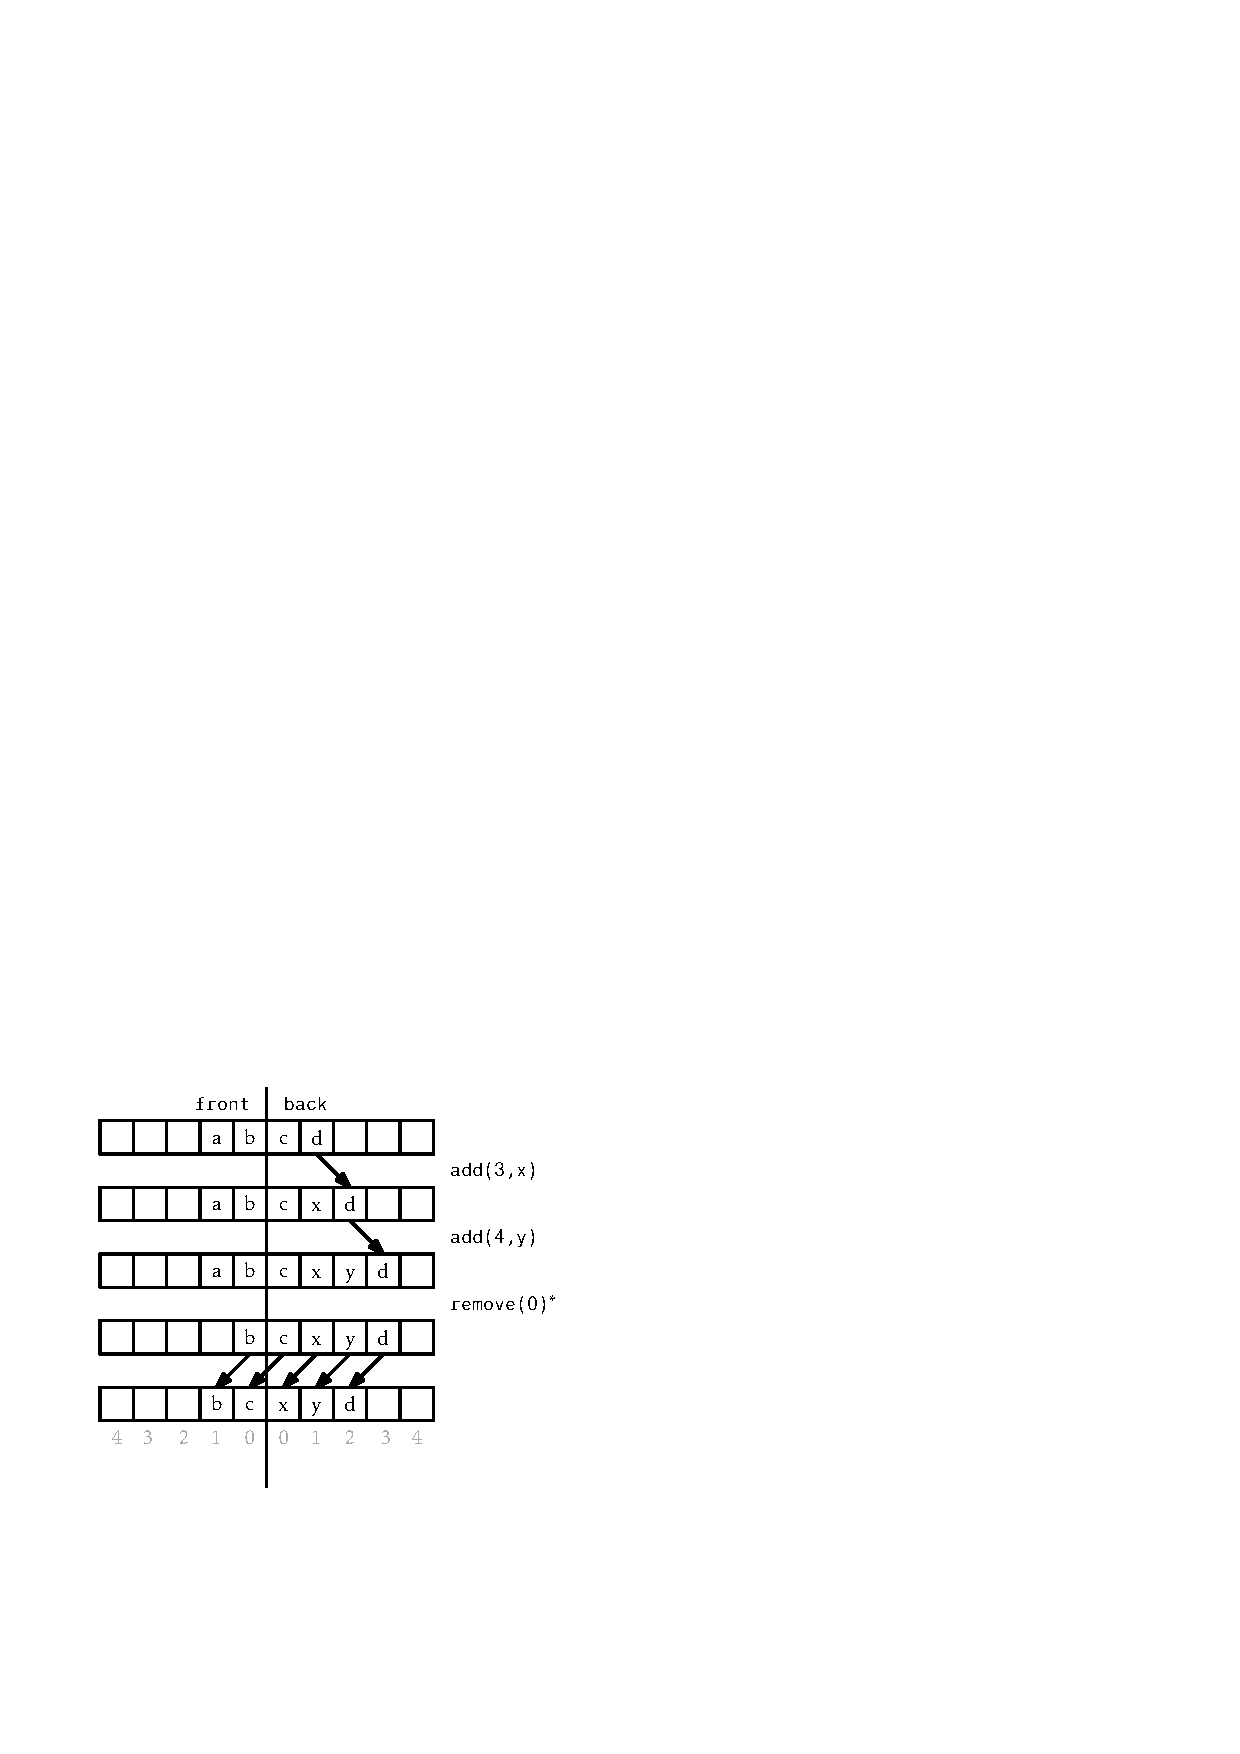
\includegraphics[scale=0.90909]{imagens/dualarraydeque}
  \end{center}
  \caption[Adding and removing in a DualArrayDeque]{Uma sequência de operações de $\ensuremath{\ensuremath{\mathrm{add}(\ensuremath{\mathit{i}},\ensuremath{\mathit{x}})}}$ and $\ensuremath{\ensuremath{\mathrm{remove}(\ensuremath{\mathit{i}})}}$ em uma
  DualArrayDeque.}

\end{figure}
\end{frame}

\begin{frame}
\frametitle{$add(i,x)$}
\begin{oframed}
\begin{flushleft}
\hspace*{1em} $\ensuremath{\mathrm{add}(\ensuremath{\mathit{i}}, \ensuremath{\mathit{x}})}$\\
\hspace*{1em} \hspace*{1em} {\color{black} \textbf{if}} $\ensuremath{\ensuremath{\mathit{i}} < \ensuremath{\mathit{front}}.\mathrm{size}()}$ {\color{black} \textbf{then}} \\
\hspace*{1em} \hspace*{1em} \hspace*{1em} $\ensuremath{\ensuremath{\mathit{front}}.\mathrm{add}(\ensuremath{\mathit{front}}.\mathrm{size}()-\ensuremath{\mathit{i}}, x})$\\
\hspace*{1em} \hspace*{1em} {\color{black} \textbf{else}} \\
\hspace*{1em} \hspace*{1em} \hspace*{1em} $\ensuremath{\ensuremath{\mathit{back}}.\mathrm{add}(\ensuremath{\mathit{i}}-\ensuremath{\mathit{front}}.\mathrm{size}(), x})$\\
\hspace*{1em} \hspace*{1em} $\ensuremath{\mathrm{balance}()} $\\
\end{flushleft}
\end{oframed}

$balance()$ garante que, a menos que $\ensuremath{\ensuremath{\mathrm{size}()}}<2$,
$\ensuremath{\ensuremath{\ensuremath{\mathit{front}}.\mathrm{size}()}}$ e $\ensuremath{\ensuremath{\ensuremath{\mathit{back}}.\mathrm{size}()}}$ não diferem em tamanho por um fator maior que 3.  Particularmente, $3\cdot\ensuremath{\ensuremath{\ensuremath{\mathit{front}}.\mathrm{size}()}} \ge \ensuremath{\ensuremath{\ensuremath{\mathit{back}}.\mathrm{size}()}}$ e
$3\cdot\ensuremath{\ensuremath{\ensuremath{\mathit{back}}.\mathrm{size}()}} \ge \ensuremath{\ensuremath{\ensuremath{\mathit{front}}.\mathrm{size}()}}$.
\end{frame}

\begin{frame}
\frametitle{$remove()$}
\begin{oframed}
\begin{flushleft}
\hspace*{1em} $\ensuremath{\mathrm{remove}(\ensuremath{\mathit{i}})}$\\
\hspace*{1em} \hspace*{1em} {\color{black} \textbf{if}} $\ensuremath{\ensuremath{\mathit{i}} < \ensuremath{\mathit{front}}.\mathrm{size}()}$ {\color{black} \textbf{then}} \\
\hspace*{1em} \hspace*{1em} \hspace*{1em} $\ensuremath{\ensuremath{\mathit{x}} \gets  \ensuremath{\ensuremath{\mathit{front}}.\mathrm{remove}(\ensuremath{\mathit{front}}.\mathrm{size}()-\ensuremath{\mathit{i}}-1})}$\\
\hspace*{1em} \hspace*{1em} {\color{black} \textbf{else}} \\
\hspace*{1em} \hspace*{1em} \hspace*{1em} $\ensuremath{\ensuremath{\mathit{x}} \gets  \ensuremath{\ensuremath{\mathit{back}}.\mathrm{remove}(\ensuremath{\mathit{i}}-\ensuremath{\mathit{front}}.\mathrm{size}()})}$\\
\hspace*{1em} \hspace*{1em} $\ensuremath{\mathrm{balance}()}$\\
\hspace*{1em} \hspace*{1em} {\color{black} \textbf{return}} $\ensuremath{\ensuremath{\mathit{x}}}$\\
\end{flushleft}
\end{oframed}
\end{frame}

\begin{frame}[shrink]
\frametitle{$balance()$}
\begin{oframed}
\begin{flushleft}
 $\ensuremath{\mathrm{balance}()}$\\
 \hspace*{0.5em} $\ensuremath{\ensuremath{\mathit{n}} \gets  \ensuremath{\mathrm{size}()}}$\\
 \hspace*{0.5em} $\ensuremath{\ensuremath{\mathit{mid}} \gets  \ensuremath{\ensuremath{\mathit{n}} $ div $2}}$\\
 \hspace*{0.5em} {\color{black} \textbf{if}} $\ensuremath{3\cdot \ensuremath{\mathit{front}}.\mathrm{size}() < \ensuremath{\mathit{back}}.\mathrm{size}()}$ {\color{black} \textbf{or}} $\ensuremath{3\cdot \ensuremath{\mathit{back}}.\mathrm{size}() < \ensuremath{\mathit{front}}.\mathrm{size}()}$ {\color{black} \textbf{then}} \\
\hspace*{0.5em} \hspace*{1em} $\ensuremath{\ensuremath{\mathit{f}} \gets  \ensuremath{\mathrm{\mathrm{ArrayStack}}()}}$\\
\hspace*{0.5em} \hspace*{1em} {\color{black} \textbf{for}} $\ensuremath{i}$ {\color{black} \textbf{in}} $\ensuremath{0,1,2,\ldots,\ensuremath{\mathit{mid}}-1}$ {\color{black} \textbf{do}} \\
\hspace*{0.5em} \hspace*{1em} \hspace*{1em} $\ensuremath{\ensuremath{\mathit{f}}.\mathrm{add}(\ensuremath{\mathit{i}}, \mathrm{get}(\ensuremath{\mathit{mid}}-\ensuremath{\mathit{i}}-1)})$\\
\hspace*{0.5em} \hspace*{1em} $\ensuremath{\ensuremath{\mathit{b}} \gets  \ensuremath{\mathrm{\mathrm{ArrayStack}}()}}$\\
\hspace*{0.5em} \hspace*{1em} {\color{black} \textbf{for}} $\ensuremath{i}$ {\color{black} \textbf{in}} $\ensuremath{0,1,2,\ldots,\ensuremath{\mathit{n}}-\ensuremath{\mathit{mid}}-1}$ {\color{black} \textbf{do}} \\
\hspace*{0.5em} \hspace*{1em} \hspace*{1em} $\ensuremath{\ensuremath{\mathit{b}}.\mathrm{add}(\ensuremath{\mathit{i}}, \mathrm{get}(\ensuremath{\mathit{mid}}+\ensuremath{\mathit{i}})})$ \\
\hspace*{0.5em} \hspace*{1em} $\ensuremath{\ensuremath{\mathit{front}} \gets  \ensuremath{f}}$\\
\hspace*{0.5em} \hspace*{1em} $\ensuremath{\ensuremath{\mathit{back}} \gets  \ensuremath{b}}$\\
\end{flushleft}
\end{oframed}
\end{frame}

\subsection{2.6 RootishArrayStack}
\begin{frame}
\frametitle{RootishArrayStack}
Uma RootishArrayStack
armazena $n$ elementos usando $O(\sqrt{\ensuremath{\ensuremath{\ensuremath{\mathit{n}}}}})$ arrays.  Nestes arrays, pelo menos
 $O(\sqrt{\ensuremath{\ensuremath{\ensuremath{\mathit{n}}}}})$ posições do array estão vazias em qualquer momento.  Todo espaço restante é usado para armazenar dados.  Assim, estas estruturas desperdiçam no máximo $O(\sqrt{\ensuremath{\ensuremath{\ensuremath{\mathit{n}}}}})$ do espaço quando estão armazenando elementos $\ensuremath{\ensuremath{\ensuremath{\mathit{n}}}}$
elementos.
\end{frame}

\begin{frame}
\frametitle{RootishArrayStack}
\begin{figure}
  \begin{center}
    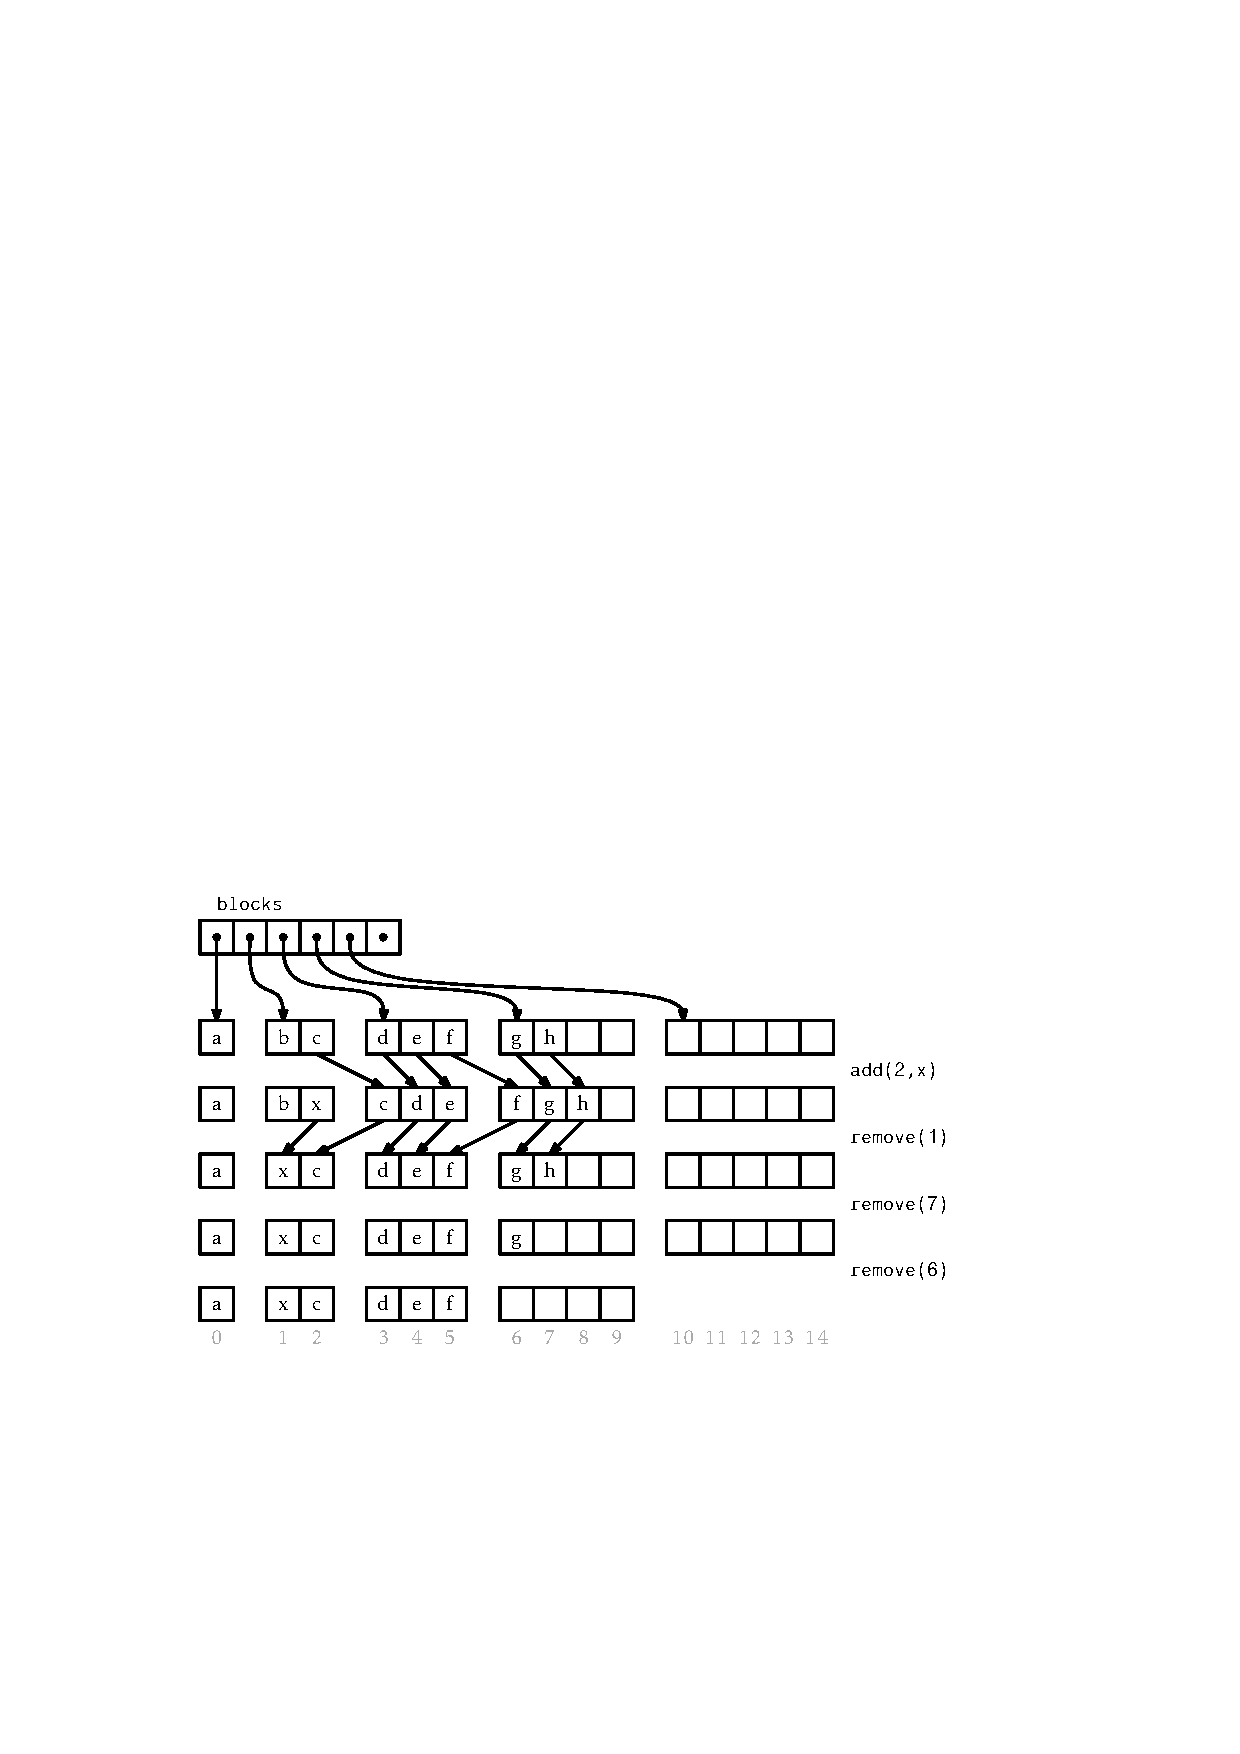
\includegraphics[width=\textwidth]{imagens/rootisharraystack}
  \end{center}

\end{figure}
\end{frame}

\begin{frame}
\frametitle{$initialize()$}
\begin{oframed}
\begin{flushleft}
\hspace*{1em} $\ensuremath{\mathrm{initialize}()}$\\
\hspace*{1em} \hspace*{1em} $\ensuremath{\ensuremath{\mathit{n}} \gets  \ensuremath{0}}$\\
\hspace*{1em} \hspace*{1em} $\ensuremath{\ensuremath{\mathit{blocks}} \gets  \ensuremath{\mathrm{\mathrm{ArrayStack}}()}}$\\
\end{flushleft}
\end{oframed}
\end{frame}

\begin{frame}


O elemento da lista com índice 0 é armazenado no bloco 0,
os elementos com índices 1 e 2 são armazenados no bloco 1, os elementos com índices 3, 4, e 5 são armazenados no bloco 2, e assim por diante.  

Se o índice \ensuremath{\ensuremath{\ensuremath{\mathit{i}}}} está no bloco \ensuremath{\ensuremath{\ensuremath{\mathit{b}}}}, então o número de elementos nos blocos
$0,\ldots,\ensuremath{\ensuremath{\ensuremath{\mathit{b}}}}-1$ é $\ensuremath{\ensuremath{\ensuremath{\mathit{b}}}}(\ensuremath{\ensuremath{\ensuremath{\mathit{b}}}}+1)/2$.  Assim, \ensuremath{\ensuremath{\ensuremath{\mathit{i}}}} está armazenado na posição
\[
     \ensuremath{\ensuremath{\ensuremath{\mathit{j}}}} = \ensuremath{\ensuremath{\ensuremath{\mathit{i}}}} - \ensuremath{\ensuremath{\ensuremath{\mathit{b}}}}(\ensuremath{\ensuremath{\ensuremath{\mathit{b}}}}+1)/2
\]
dentro do bloco \ensuremath{\ensuremath{\ensuremath{\mathit{b}}}}. 

\end{frame}

\begin{frame}
\frametitle{Cálculo de $b$}
O número de elementos que possuem índices menores que ou iguais a \ensuremath{\ensuremath{\ensuremath{\mathit{i}}}} é $\ensuremath{\ensuremath{\ensuremath{\mathit{i}}}}+1$.  Por outro lado, o número de elementos
nos blocos $0,\ldots,b$ é $(\ensuremath{\ensuremath{\ensuremath{\mathit{b}}}}+1)(\ensuremath{\ensuremath{\ensuremath{\mathit{b}}}}+2)/2$.  Assim, \ensuremath{\ensuremath{\ensuremath{\mathit{b}}}} é o menor inteiro tal que
\[
    (\ensuremath{\ensuremath{\ensuremath{\mathit{b}}}}+1)(\ensuremath{\ensuremath{\ensuremath{\mathit{b}}}}+2)/2 \ge \ensuremath{\ensuremath{\ensuremath{\mathit{i}}}}+1 \enspace .
\]
Podemos escrever esta equação como
\[
    \ensuremath{\ensuremath{\ensuremath{\mathit{b}}}}^2 + 3\ensuremath{\ensuremath{\ensuremath{\mathit{b}}}} - 2\ensuremath{\ensuremath{\ensuremath{\mathit{i}}}} \ge  0 \enspace .
\]
\end{frame}
\begin{frame}
\frametitle{$i2b()$}
A equação quadrática correspondente é $\ensuremath{\ensuremath{\ensuremath{\mathit{b}}}}^2 + 3\ensuremath{\ensuremath{\ensuremath{\mathit{b}}}} - 2\ensuremath{\ensuremath{\ensuremath{\mathit{i}}}} =  0$ que possui duas soluções: $\ensuremath{\ensuremath{\ensuremath{\mathit{b}}}}=(-3 + \sqrt{9+8\ensuremath{\ensuremath{\ensuremath{\mathit{i}}}}}) / 2$ e $\ensuremath{\ensuremath{\ensuremath{\mathit{b}}}}=(-3 - \sqrt{9+8\ensuremath{\ensuremath{\ensuremath{\mathit{i}}}}}) / 2$.

Assim, obtemos a solução $\ensuremath{\ensuremath{\ensuremath{\mathit{b}}}} = (-3 +
\sqrt{9+8i}) / 2$.  Procuramos simplesmente o menor inteiro  $\ensuremath{\ensuremath{\ensuremath{\mathit{b}}}}$ tal que 
$\ensuremath{\ensuremath{\ensuremath{\mathit{b}}}} \ge (-3 + \sqrt{9+8i}) / 2$.  Isto é simplesmente
\[
   \ensuremath{\ensuremath{\ensuremath{\mathit{b}}}} = \left\lceil(-3 + \sqrt{9+8i}) / 2\right\rceil \enspace .
\]

\begin{oframed}
\begin{flushleft}
\hspace*{1em} \ensuremath{\mathrm{i2b}(\ensuremath{\mathit{i}})}\\
\hspace*{1em} \hspace*{1em} {\color{black} \textbf{return}} \ensuremath{\mathrm{int\_value}(\mathrm{ceil}((-3.0 + \sqrt{9 + 8\cdot \ensuremath{\mathit{i}})}) / \ensuremath{2.0})}\\
\end{flushleft}
\end{oframed}
\end{frame}
\begin{frame}
\frametitle{$get()$ e $set()$}
\begin{oframed}
\begin{flushleft}
\hspace*{1em} \ensuremath{\mathrm{get}(\ensuremath{\mathit{i}})}\\

\hspace*{1em} \hspace*{1em} \ensuremath{\ensuremath{\mathit{b}} \gets  \ensuremath{\mathrm{i2b}(\ensuremath{\mathit{i}})}}\\
\hspace*{1em} \hspace*{1em} \ensuremath{\ensuremath{\mathit{j}} \gets  \ensuremath{\ensuremath{\mathit{i}} - \ensuremath{\mathit{b}}\cdot (\ensuremath{\mathit{b}}+1)/2}}\\
\hspace*{1em} \hspace*{1em} {\color{black} \textbf{return}} \ensuremath{\ensuremath{\mathit{blocks}}.\mathrm{get}(\ensuremath{\mathit{b}})[\ensuremath{\mathit{j}}]}\\
\ \\
\hspace*{1em} \ensuremath{\mathrm{set}(\ensuremath{\mathit{i}}, \ensuremath{\mathit{x}})}\\

\hspace*{1em} \hspace*{1em} \ensuremath{\ensuremath{\mathit{b}} \gets  \ensuremath{\mathrm{i2b}(\ensuremath{\mathit{i}})}}\\
\hspace*{1em} \hspace*{1em} \ensuremath{\ensuremath{\mathit{j}} \gets  \ensuremath{\ensuremath{\mathit{i}} - \ensuremath{\mathit{b}}\cdot (\ensuremath{\mathit{b}}+1)/2}}\\
\hspace*{1em} \hspace*{1em} \ensuremath{\ensuremath{\mathit{y}} \gets  \ensuremath{\ensuremath{\mathit{blocks}}.\mathrm{get}(\ensuremath{\mathit{b}})[\ensuremath{\mathit{j}}]}}\\
\hspace*{1em} \hspace*{1em} \ensuremath{\ensuremath{\mathit{blocks}}.\ensuremath{\mathrm{get}(\ensuremath{\mathit{b}})[\ensuremath{\mathit{j}}]} \gets  \ensuremath{x}}\\
\hspace*{1em} \hspace*{1em} {\color{black} \textbf{return}} \ensuremath{\ensuremath{\mathit{y}}}\\
\end{flushleft}
\end{oframed}
\end{frame}
\begin{frame}
\frametitle{$add()$}
\begin{oframed}
\begin{flushleft}
\hspace*{1em} \ensuremath{\mathrm{add}(\ensuremath{\mathit{i}}, \ensuremath{\mathit{x}})}\\

\hspace*{1em} \hspace*{1em} \ensuremath{\ensuremath{\mathit{r}} \gets  \ensuremath{\ensuremath{\mathit{blocks}}.\mathrm{size}()}}\\
\hspace*{1em} \hspace*{1em} {\color{black} \textbf{if}} \ensuremath{\ensuremath{\mathit{r}}\cdot (\ensuremath{\mathit{r}}+1)/2 < \ensuremath{\mathit{n}} + 1} {\color{black} \textbf{then}}  \ensuremath{\mathrm{grow}()}\\
\hspace*{1em} \hspace*{1em} \ensuremath{\ensuremath{\mathit{n}} \gets  \ensuremath{\ensuremath{\mathit{n}} + 1}}\\
\hspace*{1em} \hspace*{1em} {\color{black} \textbf{for}} \ensuremath{j} {\color{black} \textbf{in}} \ensuremath{\ensuremath{\mathit{n}}-1,\ensuremath{\mathit{n}}-2,\ensuremath{\mathit{n}}-3,\ldots,\ensuremath{\mathit{i}}+1} {\color{black} \textbf{do}} \\
\hspace*{1em} \hspace*{1em} \hspace*{1em} \ensuremath{\mathrm{set}(\ensuremath{\mathit{j}}, \mathrm{get}(\ensuremath{\mathit{j}}-1)})\\
\hspace*{1em} \hspace*{1em} \ensuremath{\mathrm{set}(\ensuremath{\mathit{i}}, \ensuremath{\mathit{x}})}\\
\end{flushleft}
\end{oframed}
\end{frame}
\begin{frame}
\frametitle{$grow()$}
\begin{oframed}
\begin{flushleft}
\hspace*{1em} \ensuremath{\mathrm{grow}()}\\
\hspace*{1em} \hspace*{1em} \ensuremath{\ensuremath{\mathit{blocks}}.\mathrm{append}(\mathrm{new\_array}(\ensuremath{\mathit{blocks}}.\mathrm{size}()+1}))\\
\end{flushleft}
\end{oframed}
\end{frame}
\begin{frame}
\begin{oframed}
\frametitle{$remove()$}
\begin{flushleft}
\hspace*{1em} \ensuremath{\mathrm{remove}(\ensuremath{\mathit{i}})}\\

\hspace*{1em} \hspace*{1em} \ensuremath{\ensuremath{\mathit{x}} \gets  \ensuremath{\mathrm{get}(\ensuremath{\mathit{i}})}}\\
\hspace*{1em} \hspace*{1em} {\color{black} \textbf{for}} \ensuremath{j} {\color{black} \textbf{in}} \ensuremath{\ensuremath{\mathit{i}},\ensuremath{\mathit{i}}+1,\ensuremath{\mathit{i}}+2,\ldots,\ensuremath{\mathit{n}}-2} {\color{black} \textbf{do}} \\
\hspace*{1em} \hspace*{1em} \hspace*{1em} \ensuremath{\mathrm{set}(\ensuremath{\mathit{j}}, \mathrm{get}(\ensuremath{\mathit{j}}+1)})\\
\hspace*{1em} \hspace*{1em} \ensuremath{\ensuremath{\mathit{n}} \gets  \ensuremath{\ensuremath{\mathit{n}} - 1}}\\
\hspace*{1em} \hspace*{1em} \ensuremath{\ensuremath{\mathit{r}} \gets  \ensuremath{\ensuremath{\mathit{blocks}}.\mathrm{size}()}}\\
\hspace*{1em} \hspace*{1em} {\color{black} \textbf{if}} \ensuremath{(\ensuremath{\mathit{r}}-2)\cdot (\ensuremath{\mathit{r}}-1)/2 \ge n} {\color{black} \textbf{then}}  \ensuremath{\mathrm{shrink}()}\\
\hspace*{1em} \hspace*{1em} {\color{black} \textbf{return}} \ensuremath{\ensuremath{\mathit{x}}}\\
\end{flushleft}
\end{oframed}
\end{frame}
\begin{frame}
\frametitle{$shrink()$}
\begin{oframed}
\begin{flushleft}
\hspace*{1em} \ensuremath{\mathrm{shrink}()}\\
\hspace*{1em} \hspace*{1em} \ensuremath{\ensuremath{\mathit{r}} \gets  \ensuremath{\ensuremath{\mathit{blocks}}.\mathrm{size}()}}\\
\hspace*{1em} \hspace*{1em} {\color{black} \textbf{while}} \ensuremath{\ensuremath{\mathit{r}} > 0} {\color{black} \textbf{and}} \ensuremath{(\ensuremath{\mathit{r}}-2)\cdot (\ensuremath{\mathit{r}}-1)/2 \ge n} {\color{black} \textbf{do}} \\
\hspace*{1em} \hspace*{1em} \hspace*{1em} \ensuremath{\ensuremath{\mathit{blocks}}.\mathrm{remove}(\ensuremath{\mathit{blocks}}.\mathrm{size}()-1})\\
\hspace*{1em} \hspace*{1em} \hspace*{1em} \ensuremath{\ensuremath{\mathit{r}} \gets  \ensuremath{\ensuremath{\mathit{r}} - 1}}\\
\end{flushleft}
\end{oframed}
\end{frame}

\subsection{2.7 Exercícios}
\begin{frame}
\frametitle{2.7 Exercícios}
1. O método de Lista $add\_all(i,c)$ insere todos os elementos de uma coleção $c$ na posição $i$  da lista.  (O método $add(i,x)$ é um caso especial onde $c=x$.)  Explique por que, para as estruturas desta aula, não seria eficiente implementar $add\_all(i,c)$ com chamadas repetidas a add(i,x).  Projete e implemente uma forma mais eficiente de implementação.
\end{frame}



\begin{frame}
FIM
\end{frame}
\end{document}
